\documentclass[a4paper,11pt,twoside]{book}			
\usepackage[utf8]{inputenc}                             
\usepackage[italian]{babel}
\usepackage{lipsum}								
\usepackage{listings}							
\usepackage{url}								
\usepackage{graphicx}							
\usepackage{geometry}						
\usepackage[dvipsnames]{xcolor} 				
\usepackage[hidelinks]{hyperref}		
\usepackage{chngpage}
\usepackage{multicol}
\usepackage{caption}
\usepackage{subcaption}

\usepackage{authblk}
\renewcommand\Authand{ e }
		
\geometry{a4paper,top=2cm,bottom=2cm,left=3cm,right=3cm,heightrounded,bindingoffset=10mm}
\raggedbottom									

\lstset{language=Java,						
	showspaces=false,
	showtabs=false,
	breaklines=true,
	showstringspaces=false,
	breakatwhitespace=true,
	commentstyle=\color{ForestGreen},
	keywordstyle=\color{blue},
	stringstyle=\color{red},
	identifierstyle=\color{Gray},
	basicstyle=\small\ttfamily
}

\title{Interazione Uomo Macchina per Informatici}
\author[1]{Daniele Mazzei, Dipartimento di Informatica Università di Pisa}
\date{A.A. 2020/2021}

\begin{document}

\maketitle

\tableofcontents

\chapter{Introduzione}

Negli ultimi anni il ruolo degli informatici \`e decisamente cambiato. Per anni l'informatico \`e stato chiuso in uno sgabuzzino ad interagire in
solitudine con una tastiera, bevendo bibite gassate mentre qualcuno gli diceva che cosa serviva (o almeno era convinto di sapere cosa servisse)
all'azienda per crescere.

Poi sono arrivati Internet, gli smartphone, la banda larga e l'Internet delle cose (IOT) e tutto \`e cambiato. 

Oggi gli informatici sono diventati le nuove star! 

Il mondo \`e ormai tecnocratico e le nuove soluzioni informatiche e tecnologiche hanno la capacit\`a di mutare la vita delle persone e gli andamenti
dell'economia in tempi così veloci da far rabbrividire.

Tuttavia, l'informatico \`e rimasto (spesso) in termini di attitudine e di bagaglio culturale lo stesso di prima. Li abbiamo fatti uscire dagli
sgabuzzini, abbiamo messo loro una giacca sopra la maglietta di Star Wars e li abbiamo spediti sui palchi dei tecnoeventi a fare pitch.

\`E chiaro che le competenze tecniche siano il bagaglio fondamentale per un informatico, ma in un epoca in cui le scelte degli informatici hanno
la potenzialit\`a di cambiare la vita delle persone non si può più prescindere da far capire agli informatici che cosa accade ad una persona ``normale"
(un non informatico, un babbano) quando interagisce con un software o con un sistema tecnologico in generale. 

Per troppi anni gli informatici hanno potuto limitarsi a sviluppare per i loro simili o al massimo per i loro capi. Ora che il frutto del lavoro
degli scienziati dell'informazione \`e destinato alle masse \`e arrivato il momento che gli informatici studino anche i principi fondamentali
dell'interazione uomo-macchina e uomo-computer.

Questo corso \`e una trattazione adattata per informatici delle teorie di human computer (HCI) e human machine interaction (HMI) [interazione
uomo-computer e interazione uomo-macchina]. 

Questo corso \`e ispirato alla teoria dell'interazione del Prof. Donald Norman ed in particolare, queste dispense sono in parte un adattamento didattico
del libro ``La caffettiera del masochista" di Donald Norman, pubblicato in Italia da Giunti e disponibile in lingua originale come ``The design of
everyday things, D. Norman". Consiglio di acquistare il libro per avere una trattazione con taglio più narrativo e sicuramente più esteso ed
approfondito di quanto qui riportato.

Nel corso verranno trattati anche aspetti relativi all'Internet delle cose e alle interazioni con robot e altri sistemi ``smart". Questi aspetti
legati all'interazione con oggetti smart sono anch'essi ispirati agli studi di Norman e sono ampiamente trattati nel libro
``Il Computer Invisibile, D. Norman", pubblicato in Italia da Apogeo.

L'obiettivo di questo corso \`e quindi quello di fornire agli studenti del corso di laurea in Informatica gli strumenti necessari a comprendere e
gestire il processo di sviluppo delle interfacce e dei prodotti interattivi. Questo corso ambisce quindi a spostare l'informatico dal suo tipico
ruolo di sviluppatore per farlo diventare un progettista non solo del ``codice" ma del prodotto nel suo insieme.

Nel corso parler\`o spesso di ``prodotto" (nei termini di questo corso, viene definito come qualsiasi cosa un utente usi), ``business",
``acquisto" e altri termini legati al mondo della vendita, dell'economia e del mercato. Questo perch\'e l'informatico deve a mio parere sviluppare
una consapevolezza fondamentale per il suo lavoro:

\vspace{\baselineskip}
\textbf{un prodotto che nessuno compra \`e un prodotto inutile}.
\vspace{\baselineskip}

Non importa quanto geniale sia il codice che avete scritto o rivoluzionario il sistema che avete implementato, se non vi curerete di far s\`i che questo
artefatto venga apprezzato (e quindi utilizzato dalle persone) la vostra creazione, geniale o stupida che sia, morir\`a dentro il vostro computer.

Per comprendere appieno la definizione di prodotto, si prende come esempio ``Google" (motore di ricerca): \`e gratuito, \`e un prodotto che viene
usato come servizio e ha una certa strategia di remunerazione.

\vfill
\textit{Queste dispense derivano dagli appunti di Simone Pepi e Francesco Iannelli pubblicati su \href{https://github.com/unipi-notes/HMI_Notes-2019-20}
{\underline{GitHub}} e relativi all' A.A 19/20}.

\textbf{Queste dispense sono ad esclusivo uso degli studenti del corso di Programmazione di Interfacce dell'Universit\`a di Pisa. \`E
vietata la divulgazione, copia o riproduzione in qualsiasi forma}.
 %introduzione
\chapter{Progettare l'Interazione fra Uomo e Macchina}

La rivoluzione tecnologica degli ultimi anni ha portato a parlare molto di User Experience Design, User Interface Design, Interaction Design etc.

\vspace{\baselineskip}
Cosa si intende con il termine \textbf{Design}?
\vspace{\baselineskip}

In Italiano tendiamo ad usare il termine design per riferirci sia al processo di progettazione che al risultato stesso di questo processo:
\begin{flushleft}
    \textit{(processo)``...\`E stato avviato il design dell'interfaccia grafica"}

    \textit{(risultato del processo)``...Ecco il design dell'interfaccia grafica pronto per essere implementato"}
\end{flushleft}

Per design si intende quindi \textbf{sia il processo di progettazione e pianificazione sia il risultato di questo processo}.
 
\`E importante notare che nel mondo del design, ed in particolare nel design industriale, si approccia alla risoluzione dei problemi e alla progettazione
con una forma mentis molto diversa rispetto a quella ``computazionale" tipica del mondo informatico.

Nel 2006 Jeannette Wing, direttrice del Dipartimento di informatica della Carnegie Mellon University, formulò la seguente definizione di pensiero
computazionale:
\textit{``il pensiero computazionale è un processo di formulazione di problemi e di soluzioni in una forma che sia eseguibile da un agente che processi
informazioni."}

Il pensiero computazionale consiste nel pensare a diversi livelli di astrazione in modo tale da individuare sottoproblemi risolvibili con una serie finita
di azioni atomiche (i.e. risolvibile da un ``algoritmo"): è quindi un processo mentale che consente di risolvere problemi di varia natura seguendo
metodi e strumenti specifici, pianificando una strategia; abitua al rigore e quindi rende possibili gli atti creativi. Permette di interagire con
persone e strumenti, di fruire delle potenzialità delle macchine quali oggetti capaci di compensare le lentezze o l’imprecisione dell’uomo, se ben
programmati.

Nel modo del design invece, la progettazione è tipicamente affrontata in maniera globale. L'obiettivo principale del design di prodotto non è
necessariamente quello di trovare una soluzione al problema specifico ma è piuttosto quella di \textbf{comprendere il problema stesso nel suo insieme}.

Nel mondo del design il primo passo è sempre quello di capire perché il problema esiste e solo dopo aver appurato che l'origine di un problema non può
essere eliminata o mitigata ci si adopera per cercare di risolverlo nello specifico. Viceversa, l'informatico medio non appena si trova davanti ad un
problema, apre il proprio editor di testo e inizia a scrivere un algoritmo per cercare di risolverlo senza neanche chiedersi se il problema che si sta
affrontando esiste veramente.

\textit{Cosa vuol dire ``se il problema esiste veramente?"}
\vspace{\baselineskip}

George Berkeley, un filosofo irlandese del '700 sosteneva che gli oggetti esistono solo in quanto percepiti. Dunque, se un albero cade in una foresta
e nessuno lo sente, non fa rumore.

Estesa al mondo dell'interazione uomo-macchina e dello sviluppo prodotto in generale, la filosofia di Berkeley ci dice quindi che se un problema non è
percepito da un utente allora quel problema non esiste. Nel design dell'interazione e quindi dell'esperienza utente l'obiettivo primo è (o almeno, dovrebbe
essere) quello di avere un utente soddisfatto non un software teoricamente perfetto or super-ricco di funzionalità.

%Si evince quindi che, nel pensiero computazionale si raggiunge un risultato quando si ottiene un algoritmo che è in grado di risolvere il problema dato.
%Questo problema per poter essere risolto tramite un algoritmo deve essere matematicamente descrivibile e deve avere ingressi, uscite, vincoli e requisiti
%chiari, definiti e immutabili (nella loro definizione).
 
Questo può portare a situazioni che dal punto di vista informatico sono percepite come assurde. Nel design di prodotto ci si trova infatti spesso
costretti a modificare i requirement e le specifiche di prodotto per andare in contro alle esigenze degli utenti e sacrificando funzionalità tecniche
e qualità dell'implementazione software.
Trovare il corretto bilanciamento fra esperienza utente, funzionalità e qualità tecnica è la parte più complessa dell'intero processo di sviluppo
prodotto. Nei prossimi capitoli introdurremo delle tecniche e dei processi atti a gestire questo processo in maniera scientifica e strutturata.
 
%e cioè assurda (dal punto di vista informatico) condizione in cui si modificano gli obbiettivi dello sviluppo al fine di assolvere alle esigenze
%dell'utente in termini di esperienza.
 
Questo processo antropocentrico di adattamento del software alle esigenze dell'utente piuttosto che al virtuosismo tecnico è spesso vissuto dalla maggior
parte degli informatici come un'assurda violenza. Per questo motivo è molto importante che gli informatici studino i principi del design, perché il mondo
del design antropocentrico è per i tecnici tipicamente molto molto complicato da metabolizzare in quanto distante dal pensiero computazionale.

\`E importante evidenziare che design dell'interazione e pensiero computazionale non sono mutualmente esclusivi, anzi. \`E nell'unione dei due e
nell'integrazione dei due processi di studio e progettazione che nascono prodotti di successo e software di qualità.
\vspace{\baselineskip}

%Ogni cosa con cui abbiamo quotidianamente a che fare è il risultato di un processo di design; una lampada, una strada, una casa. Nella progettazione
%di oggetti interattivi e interfacce utente però non possiamo limitarci alla progettazione puramente estetica. \`E necessario infatti andare oltre
%l'aspetto fisico e la piacevolezza alla vista o al tatto di un oggetto e curarci dell'esperienza e quindi della sensazione che l'utente proverà
%nell'interagire con l'oggetto (frutto) del nostro design. Un'interfaccia molto bella e graficamente accattivante ma impossibile da utilizzare è
%sicuramente un pessimo risultato per un processo di design.

\begin{flushleft}
\textbf{ \textit{``If we want users to like our software, we should design it to behave like a likeable person: respectful, generous and helpful.''}}

\textit{Alan Cooper, software designer e programmatore, noto come ``il padre del Visual Basic"}
    
\end{flushleft}


\section{Interaction Design}
Il mondo della progettazione è diventato talmente ampio e variegato che il termine design da solo ormai non ha quasi più significato. Esistono varie sotto
discipline del design e con queste numerose professioni, metodi di lavoro, scuole di pensiero e altrettante immancabili faide e lotte fra fazioni.

Un informatico può fare a meno di conoscere al completo il mondo del design ma non può esimersi da possedere i rudimenti base del ``design
dell'interazione".

Interaction design, o progettazione dell'interazione, è l'attività di progettazione dell'interazione che avviene tra esseri umani e oggetti in generale. 

%e la fruizione di servizi e sistemi complessi in modo proficuo e soddisfacente.

L'obiettivo principale dell'interaction design è quello di rendere macchine, servizi e sistemi usabili dagli utenti per cui sono stati pensati
e realizzati e non solamente dai propri creatori. All'interno di un processo di interaction design, si investigano l'uso che verrà fatto
dell'artefatto e il target a cui esso si rivolge. Questo significa che le questioni legate agli utenti guidano il processo più di quanto non facciano
le questioni tecniche. Gli sviluppatori devono mettere al centro del processo di sviluppo i bisogni degli utenti, arrivando a realizzare un prodotto
più appropriato e maggiormente usabile. Le forze trainanti lo sviluppo di un prodotto dovrebbero essere quindi gli utenti reali e i loro bisogni e
non solo le tecnologie.


%Uno dei principali e normalmente più visibili campi di intervento è la progettazione delle interfacce, attraverso cui avviene l'interazione uomo-macchina.

Nel nostro caso ci focalizzeremo sull'interazione fra uomo e sistemi informatici e quindi andremo a lavorare nel campo dell'interazione uomo-macchina
e uomo-computer (in Inglese HMI Human-Machine Interaction e HCI Human Computer Interaction). L'obiettivo principale del HMI e HCI design è quindi
rendere possibile e facilitare al massimo, per un essere umano, l'uso e l'interazione con sistemi del mondo IT (Information Technology) quali,
calcolatori, dispositivi mobili, servizi web etc.

Interaction design, HMI e HCI sono discipline molto variegate ed ampie che spaziano dall'informatica, alla psicologia, passando per la grafica e
l'ingegneria. 

Capiamo meglio il mondo dell'Interaction design analizzando in dettaglio alcune sotto discipline del design: il \textbf{design di prodotto},
il \textbf{design dell'esperienza utente} e il \textbf{design dell'interfaccia}. 


\begin{figure}[!ht]
	\centering
	\includegraphics[scale=0.5]{immagini/interactiondesign2.png}
	\caption{Il design dell'interazione è un settore altamente interdisciplinare in cui si vanno a compenetrare diverse discipline.}
\end{figure}

Prima di entrare nel dettaglio è importante sottolineare che nessuna di queste discipline o settori della progettazione è rigidamente definite e spesso
le tre si intrecciano e vengono quindi eseguite da team multi disciplinari. Inoltre, specialmente in piccole aziende e piccoli team di sviluppo non
si riesce a separare queste attività di progettazione e quindi è estremamente importante che l'informatico moderno conosca i rudimenti di base
necessari per poter contribuire ad un team in cui vengono portate avanti anche questa tipologia di attività.


\subsection{Product Design}
Il \textbf{design di prodotto} è un processo strategico di risoluzione dei problemi che guida l'innovazione e porta a una migliore qualità della vita
attraverso prodotti, sistemi, servizi ed esperienze innovative (\textit{definizione ufficiale di disegno industriale coniata nel 2015 dalla World
Design Organization (ex ICSID). Spesso design di prodotto e design industriale sono utilizzati in modo intercambiabile}). 

Nel design di prodotto si progettano beni e servizi il cui obiettivo principale è quello di essere utilizzati da quanti più utenti possibili
migliorandone la vita; dunque, il designer (di prodotto) è colui che inventa un nuovo modo o un nuovo oggetto per fare cose che fino a ieri non si potevano
fare o si facevano in maniera più complicata.

Riassumendo, il design di prodotto è il punto di partenza dei processi di innovazione e rappresenta il punto di partenza del percorso di design
dell'interazione che stiamo esplorando; l'inventore (il designer del prodotto) si focalizza su un problema da risolvere e inventa un prodotto che
grazie alle sue caratteristiche tecniche lo permette.

Descriviamo un prodotto noto come se stessimo provando a formalizzare un processo di product design atto a reinventare un processo noto e consolidato:
ascoltare musica.

\begin{flushleft}
\textbf{Nome prodotto}: Spotify;

\textbf{Problema a cui assolve}: Ascoltare musica senza possederla;

\textbf{Tipologia di prodotto}: Servizio basato su Internet;

\textbf{Funzionalità principale}: Consentire l'ascolto di qualunque brano, su qualsiasi piattaforma senza richiedere l'acquisto di un supporto fisico
e dei diritti d'autore;

\textbf{Soluzioni esistenti}: Noleggio/prestito CD e altri supporti fisici, download di musica pirata;

\textbf{Soluzione}: Servizio di streaming basato su business model ``freemium" che di fatto rappresenta un jukebox con brani pressoché illimitati;

\textbf{Requisiti per l'utilizzo}: PC o smartphone o tablet, Connessione internet. 
\end{flushleft}

Estremizzando un po' i concetti potremmo dire che il product designer di Spotify ha terminato il suo lavoro. Quello sopra descritto è il frutto del
processo di design di prodotto che ha portato alla nascita di un servizio rivoluzionario come Spotify. Non c'è tanto altro da aggiungere per descrivere
il concetto che sta alla base del prodotto e quindi l'innovazione che esso introduce.

\begin{figure}[!h]
	\centering
	\includegraphics{immagini/spotifycanvas.png}
	\caption{Business model canvas di Spotify (\href{http://lumosbusiness.com/business-model-canvas-spotify/}{Fonte}).}
\end{figure}

\`E chiaro però che questo nuovo prodotto potrebbe essere realizzato in tanti modi e che sarà proprio il modo in cui viene costruito a decretarne il
successo o il fallimento del prodotto. Questo perché non basta un'idea per fare un prodotto di successo, ci vuole un lungo e complicato processo di
progettazione che vada oltre l'idea e metta al centro l'utente, i suo bisogni e le sue aspettative: inventare qualcosa che non esiste ma che non
risulta davvero utilizzabile per gli utenti non è garanzia di successo; spesso i prodotti rivoluzionari sono quelli che reinventano cose già
esistenti offrendo una esperienza utente migliore (si veda l'esempio di PayPal che risolve un ``non-problema").

\subsection{User Experience Design}
Il \textbf{design dell'esperienza utente} è il processo volto ad aumentare la soddisfazione e la fedeltà del cliente migliorando l'usabilità, la
facilità d'uso e il piacere fornito nell'interazione tra il cliente e il prodotto. La progettazione dell'esperienza utente comprende la tradizionale
progettazione dell'interazione uomo-macchina e la estende integrandola con tutti gli aspetti di business, marketing e sviluppo prodotto necessari per
garantire il successo del prodotto e/o servizio.

%L'esperienza utente è qualsiasi aspetto di un'interazione della persona con un dato sistema informatico e interattivo. La progettazione dell'esperienza
%studia il prodotto nel suo insieme trattando aspetti legati all'interfaccia, alla grafica, alla progettazione industriale e all'interazione fisica e
%manuale.

Ogni prodotto durante l'utilizzo da parte di un utente porta a far vivere un esperienza e di conseguenza si dice abbia una sua ``user experience".
Ovviamente, la user experience non è una proprietà del prodotto in se ma piuttosto una relazione che intercorre fra il prodotto ed uno specifico utente.
Il tema delle relazioni e della relatività delle esperienze verrà meglio affrontato nei capitoli successivi. 

%Per ora limitiamoci a sottolineare che non è possibile progettare l'esperienza utente ma si progetta \textbf{per} l'esperienza utente.

Lo \textbf{UX Designer} ha l'obiettivo di far vivere all'utente del suo prodotto la miglior esperienza possibile, evitando che l'oggetto
induca nell'utente sensazioni di frustrazione e delusione. Spesso si tende a dire che si ``progetta l'esperienza utente". In realtà è impossibile
progettare l'esperienza utente perché ogni utente è diverso dall'altro e illusorio pensare che chiunque durante l'utilizzo del prodotto si
comporti alla stessa maniera e in particolare si comporti esattamente come il progettista ha ipotizzato. \`E corretto dire che si
``progetta \textbf{per} l'esperienza utente".

Come vedremo nei capitoli successivi, lo studio e la progettazione dell'esperienza utente partono sempre dalla analisi e comprensione delle esigenze
dell'utente e non dalle specifiche funzionali di prodotto. 

\subsection{User Interaction Design}
Il Design dell'interazione ha come focus il modo in cui le persone interagiscono con la tecnologia, lo scopo è migliorare la loro comprensione di ciò
che si può fare, ciò che succede e ciò che è appena successo, basandosi su principi psicologici, tecnici ed estetici. Dallo studio della UX si crea
uno schema di interazione che poi viene passato allo \textbf{UI Designer} che ha il compito di progettare l'interfaccia utente al fine di abilitare
l'esperienza progettata.

\begin{figure}[!ht]
	\centering
	\includegraphics[scale=0.4]{immagini/uidesign.jpeg}
	\caption{Esempio di progetto di UI per una App mobile. Il wireframe riporta le linee guida per la struttura dell'interfaccia e il flusso utente
	(implementato a partire dal lavoro di UX Design) (\href{https://blog.prototypr.io/why-you-shouldnt-skip-your-wireframing-1f7a70d5c125}{Fonte}).}
\end{figure}

Lo UI designer non costruisce l'interfaccia utente, nei team numerosi questa figura è spesso un progettista grafico e non un informatico;
il suo obiettivo è quello di progettare l'aspetto estetico e la struttura dell'interfaccia così che questa durante l'utilizzo induca
l'utente nel seguire l'esperienza che è stata per lui progettata. Lo UI designer produce un wireframe, una bozza grafica dell'interfaccia e una
serie di linee guida che poi verranno seguite dagli sviluppatori (UI developer o Front-end developer) per implementare la reale interfaccia del prodotto
o servizio (ad esempio, è compito dello UI designer decidere quale sarà la posizione di un menù a tendina).

%o differente dal front-end developing: la materia progetta le guidelines che istruiscono il developer su come creare al meglio una UI.

%Non è sbagliato considerare lo UI Design come \textbf{sotto area} dello UX Desing.

\begin{figure}[!h]
	\centering
	\includegraphics[width=\textwidth]{immagini/UX_and_UI.png}
	\caption{Flusso di lavoro e ruoli necessari per lo sviluppo di un prodotto
	(\href{https://www.crayondata.com/blog/the-difference-between-ui-and-ux/}{Fonte}).}
\end{figure}

Il processo di Product Design è un percorso strutturato che include varie figure e discipline. In grandi team questi step sono eseguiti
tipicamente da diverse persone e team ma spesso nella media e piccola impresa o startup questo percorso deve poter essere seguito in autonomia da una
o al massimo due figure.

L'interfaccia vera e propria viene implementata solo alla fine del percorso di progettazione da figure con profilo tecnico informatico
(Front End Developer o UI Developer). Queste figure devono essere in grado di comprendere le richieste provenienti dagli step di progettazione
precedenti e possedere i rudimenti base dell'Interaction Design e delle relative sotto discipline.


 %Progettare l'Interazione fra Uomo e Macchina
\chapter{Human Centered Design}

\textit{I progettisti devono produrre cose che soddisfino i bisogni della gente, in termini di funzioni, facilità d’uso e gratificazione emotiva. In altre
parole, il design (di prodotto) deve essere pensato come un’esperienza totale (per l'utente).}

[Donald Norman — La caffettiera del masochista]
\vspace{\baselineskip}

Le persone sono sempre più frustate dalla complessità degli oggetti quotidiani. Dalla complessità sempre maggiore del cruscotto dell'auto, dalla lavatrice
piena di incomprensibili funzioni e pulsanti, dalla crescente automazione della casa, e dalla continua proliferazione di funzioni che i progettisti
aggiungono con orgoglio ad ogni nuova versione dei loro prodotti.

La vita della maggior parte degli utenti è ormai diventata una battaglia quotidiana per la sopravvivenza alla invadente e iper-funzionale
tecnologia. %tutti i giorni sembra a volte una battaglia infinita contro la confusione, gli errori continui, la frustrazione e un ciclo
%interminabile di aggiornamenti e manutenzioni degli apparecchi.

Questo problema origina direttamente dalla modalità con la quale oggigiorno vengono progettati gli oggetti quotidiani ed in particolare quelli tecnologici.
Le macchine (computer) hanno una modalità di funzionamento logica, dovuta all'algoritmo che il progettista ha sviluppato come anima della macchina.
Noi umani invece siamo tutt'altro che logici e razionali, siamo intuitivi, flessibili, versatili e curiosi. \`E chiaro che nell'interazione
uomo-macchina si va a creare una relazione fra specie diverse che hanno modalità di pensiero e di funzionamento opposte.

Gli ingegneri e gli informatici, orgogliosi dei loro progressi tecnologici, hanno preteso da sempre che gli umani si adattassero alle loro macchine.
Le macchine sono viste come un elemento di orgoglio che rappresenta il progresso e chi non è in grado di capirle è retrogrado, vecchio e a volte anche
un po' stupido.

Questo approccio tecno-centrico dei progettisti ha in realtà leso lo sviluppo stesso della tecnologia dal momento che ne ha rallentato la sua diffusione
e accettazione. La maggior parte degli utenti oggi è frustrata dall'utilizzo di incomprensibili oggetti tecnologici di cui non capisce il principio
di funzionamento e dove tipicamente si limita ad utilizzare il 10\% delle funzionalità disponibili.

Le macchine hanno delle loro regole di funzionamento che sono spesso note solo ai progettisti. Quando non si seguono queste regole le cose non vanno
come previsto e l'utente si sente stupido ed incapace. La macchina è perfetta, non può sbagliare, quindi se le cose sono andate male è sicuramente colpa
dell'umano. \`E vero ma non è l'umano utente ad aver sbagliato, la colpa è del progettista!

Nel design antropocentrico si inverte il paradigma di progettazione mettendo l'utente al centro del processo. Le funzionalità del prodotto vengono dopo.
Prima ci sono i bisogni dell'utente!

Questo processo, apparentemente ovvio e banale, risulta in realtà estremamente difficile da applicare per gli informatici. I tecnici infatti amano le
funzioni e funzionalità, amano le peculiarità tecniche dei sistemi e sono spesso spinti a sviluppare nuove soluzioni non tanto per risolvere problema
ma piuttosto per soddisfazione personale di aver implementato qualcosa che prima non esisteva.

La blockchain è sicuramente un esempio di questo fenomeno. Creata per diletto da degli appassionati di crittografia, ha dato vita alla prima criptomoneta
della storia. Dopo il boom di Bitcoin e delle altre criptomonete è scoppiata la bolla blockchain dove tutti nel mondo IT hanno iniziato a dichiarare
che grazie alla blockchain si sarebbe potuto innovare in maniera radicale tantissimi settori. Ad oggi in realtà dopo aver lanciato numerosi bandi
di concorso in tutto il mondo, aver aperto fondi di investimento dedicati alle startup che utilizzano tecnologia blockchain non si è ancora trovata una
applicazione di successo, oltre alle criptomonete, che senza blockchain non sarebbe realizzabile.

Per dirla in altre parole, nessun utente ci ha chiesto di sviluppare la blockchain in quanto tale, c'era bisogno di scambiarsi denaro in maniera
alternativa e quindi sono nate le criptomonete. Ora la corsa a cercare di applicare la blockchain ad altri settori non sta funzionando perché non
esiste il problema da risolvere! Stiamo cercando un problema per una tecnologia ma bisognerebbe cercare tecnologie che risolvono problemi!

La morale di questo ragionamento è: se vogliamo progettare tecnologia per le persone dobbiamo capire sia la tecnologia che le persone. Dobbiamo
pensare a risolvere i problemi delle persone (non a crearne di nuovi perché dobbiamo bulimicamente sviluppare nuova tecnologia) e smettere di progettare
per le persone come vorremmo fossero e iniziare a farlo per come realmente sono.


\begin{figure}[!htb]
	\centering
	\includegraphics[scale=0.5]{immagini/starwars.jpg}
	\caption{La tecnologia è percepita come utile quando è possibile comunicarci per risolvere insieme problemi.}
\end{figure}

Questo vuol dire passare da un approccio tecno-centrico a uno antropocentrico. Lo human centered desing o HCD, è una \textbf{metodologia di progettazione
che parte dai bisogni, dalle capacità e dai comportamenti umani, adattando la progettazione a quei bisogni, quelle capacità e quei comportamenti}.
Lo HCD è un approccio di design specificamente orientato allo sviluppo di sistemi interattivi, con l'obiettivo di produrre sistemi utili,
altamente usabili e che si \textbf{focalizzino sull'utente}.

Il design antropocentrico è orientato all'efficienza ed all'efficacia e punta ad aumentare la soddisfazione dell'utente durante
l'utilizzo del prodotto e ad evitare il più possibile gli effetti negativi e indurre frustrazione.

\vspace{\baselineskip}
\textbf{Prima l'utente, poi le features!}.
\vspace{\baselineskip}

Lo HCD mette i bisogni, comportamenti e capacità umane prima di tutto e progetta in funzione di esse. Per questo motivo il processo HCD parte
dall'osservazione dell'utente, dei suoi comportamenti: dallo studio dei suoi bisogni per poi arrivare solo dopo all'identificazione
della tecnologia necessaria.

Il problema principale delle UI è la comunicazione fra uomo e macchina. L'interazione uomo-macchina è una forma di dialogo inter-specie; due soggetti
aventi culture, corpi e lingue diverse si trovano a dover interagire per risolvere insieme un problema che uno dei due (l'umano) ha.
%, in particolare la comunicazione dalla macchina verso l'uomo, \textbf{una buona interfaccia \textit{sa} comunicare con l'utente}.

Progettare interfacce che funzionano fintanto che le cose vanno bene è relativamente facile, ma \textbf{la comunicazione è ancora più importante
quando le cose non vanno bene}. È qui che i progettisti devono concentrare l'attenzione, sui casi in cui le cose vanno storte, non su quelli in cui
le cose funzionano secondo i piani.

Questo approccio è valido sempre, non solo nello sviluppo tecnologico. Un buon avvocato scrive un contratto in previsione di cosa potrebbe andare
male nella relazione fra le parti. Se le cose dovessero andare bene sicuramente le parti non avranno bisogno del contratto e questo verrà dimenticato
in un cassetto. Il contratto diventa utile quando qualcosa va storto e se ben fatto rende la gestione del problema molto più semplice, veloce e
potenzialmente indolore. 

\`E quindi bene focalizzare sempre l'attenzione su ciò che potrebbe andare storto durante l'interazione così da progettare accuratamente la comunicazione
e guidare l'utente verso la risoluzione del problema così da ridurre la frustrazione e la negatività verso il prodotto. 

Non bisogna aver paura che l'utente abbia problemi o che il nostro software abbia degli errori o bug, è inevitabile che questo accada. \`E importante
progettare perché l'utente venga guidato nella risoluzione e gestione dell'errore senza provare frustrazione. Avremmo così un utente soddisfatto. 

L'esperienza di utilizzo produce emozioni negli utenti, più emozioni positive (successi) l'utente avrà e migliore sarà la percezione che avrà del
nostro prodotto. \`E importante sottolineare inoltre che la memoria ha la capacità di far provare sensazioni più profonde rispetto al presente. Un
utente che di fronte ad un problema riesce a risolverlo perché ben guidato dalla tecnologia avrà memoria di un suo successo. Questo tipo di sensazioni
sono molto forti e se associate al prodotto fanno si che l'utente sviluppi empatia per il prodotto e che lo apprezzi e ne senta il bisogno.

L'obiettivo dello HCD deve dunque essere quello di \textbf{creare nell'utente empatia verso il sistema}.

%\textbf{Evitare quindi la frustrazione e aiutare nella risoluzione quando insorge un problema sono i concetti chiave dello HCD.}
%Lo HCD è una filosofia di design che parte dalla \textbf{comprensione delle persone e dei bisogni che esse intendono soddisfare}. Questa comprensione deriva dall'osservazione e dallo studio delle persone che spesso sono inconsapevoli dei loro veri bisogni e magari anche delle difficoltà che incontreranno.

\begin{figure}[!h]
	\centering
	\includegraphics[width=0.7\textwidth]{immagini/HCD.png}
\end{figure}

Riassumendo, l'HCD è una \textbf{forma di pensiero} (\textbf{NON} un'area o un metodo) compatibile con le varie discipline del design di prodotto che
abbiamo precedentemente introdotto: è infatti applicabile sia al design industriale sia alla progettazione dell'interazione o
dell'esperienza utente.

A sottolineare quanto l'HCD sia ritenuto oggigiorno fondamentale per la progettazione di sistemi destinati all'utilizzo umano, è
importante ricordare che il design antropocentrico è ormai parte della norma ISO EU.

\vspace{\baselineskip}
\textbf{ISO 9241-210: 2019 Ergonomics of human-system interaction \\Part 210: Human-centered design for interactive systems}
\\(\href{https://www.iso.org/standard/77520.html}{Fonte}).
\vspace{\baselineskip}

\textit{This document provides requirements and recommendations for human-centred design principles and activities throughout the life cycle of
computer-based interactive systems. It is intended to be used by those managing design processes, and is concerned with ways in which both hardware
and software components of interactive systems can enhance human-system interaction.}

\textit{Computer-based interactive systems vary in scale and complexity. Examples include off-the-shelf (shrink-wrap) software products, custom office
systems, process control systems, automated banking systems, Web sites and applications, and consumer products such as vending machines, mobile phones
and digital television. Throughout this document, such systems are generally referred to as products, systems or services although, for simplicity,
sometimes only one term is used. This document provides an overview of human-centred design activities. It does not provide detailed coverage of the
methods and techniques required for human-centred design, nor does it address health or safety aspects in detail. Although it addresses the planning
and management of human-centred design, it does not address all aspects of project management. }

\textit{The information in this document is intended for use by those responsible for planning and managing projects that design and develop interactive
systems. It therefore addresses technical human factors and ergonomics issues only to the extent necessary to allow such individuals to understand their
relevance and importance in the design process as a whole. It also provides a framework for human factors and usability professionals involved in
human-centred design.}

\textit{Detailed human factors/ergonomics, usability and accessibility issues are dealt with more fully in a number of standards including other parts
of ISO 9241 (see Annex A) and ISO 6385, which sets out the broad principles of ergonomics.}

Un buon processo HCD parte, come abbiamo detto, dall'osservazione dell'utente e dei suoi bisogni. Tuttavia, tale osservazione non è sempre possibile o
facile da attuare. Nei successivi capitoli analizzeremo varie tecniche di prototipazione rapida e metodi di lavoro finalizzati all'estrazione veloce di
bisogni utente e all'esecuzione rapida e a basso costo di test. 

Possiamo schematizzare un processo di HCD come un flusso continuo ed iterativo che attraversa le seguenti fasi:
\begin{figure}[!h]
	\centering
	\includegraphics[scale=0.8]{immagini/HCD-chart}
	\caption{Flusso di lavoro tipico di un processo di design antropocentrico
	(\href{https://www.usability.gov/what-and-why/user-centered-design.html}{Fonte}).}
\end{figure}
\begin{itemize}
	\itemsep-0.3em
    \item \textbf{Specificare il contesto d'uso:} identificare gli utenti che utilizzeranno il prodotto, per cosa lo utilizzeranno e sotto quale
	condizioni e vincoli;
    \item \textbf{Specificare i Requirements:} Identificare i business requirement e gli obbiettivi utente che devono essere raggiunti grazie all'utilizzo
	del software;
    \item \textbf{Progettare la soluzione:} questa fase può essere a sua volta spacchettata in sotto fasi iterative. Si passa tipicamente dadelle bozze
	a dei prototipi e poi alla soluzione;
    \item \textbf{Testare e valutare:} è fondamentale testare e valutare il sistema così da poter iniziare il ciclo sulla base dei risultati dei
	test e procedere ad uno sviluppo e miglioramento incrementale.
\end{itemize}

Per ora, al fine di inquadrare meglio la filosofia HCD nel contesto dello sviluppo software vi basti pensare che le versioni alfa e beta dei nostri
software possono diventare potenti strumenti di analisi degli utenti. Le versioni di test non servono solamente a fare debugging del codice e
delle funzioni, ma anche e soprattutto a capire che cosa fanno e come si comportano gli utenti durante l'utilizzo del nostro software.

Nello sviluppo software diventa indispensabile abilitare dei sistemi di tracking dell'utente finalizzati alla produzione di statistiche di
utilizzo. Avere zero errori (segnalazioni di bug) su una funzionalità che nessuno usa non vuol dire che questa sia perfetta ma soprattutto vuol dire
che non aveva senso implementarla e quindi non ha senso mantenerla. Viceversa, avere alti utilizzi di una funzionale che era stata pensata come opzionale
o accessoria ci deve indurre a pensare che invece gli utenti hanno trovato quel processo più utile e soddisfacente rispetto a quello che in fase di
progettazione il designer aveva pensato come ``principale" e fondamentale.

Nell'a.a. 2021/2022 non è stata trattata la sezione immediatamente successiva.


\section{Usabilità}
%Ottenere \textbf{le specifiche dello HCD} è quindi una delle parti più difficili del design stesso, al punto che il principio è quello
%\textbf{di evitare di specificare il più al lungo possibile} e procedere con ripetute approssimazioni: si esegue una specifica ad alto livello,
%se ne implementa una parte, si testa sull'utente finale e tramite il suo feedback, si modifica la parte implementata e la si testa di nuovo.
%Fatto ciò si passa, magari momentaneamente, ad implementare un'altra parte.

Secondo la norma ISO, per usabilità si intende il \textit{``grado in cui un prodotto può essere usato da particolari utenti per raggiungere
certi obiettivi con efficacia, efficienza e soddisfazione in uno specifico contesto d’uso".} 

Sul \href{https://www.agid.gov.it/it/design-servizi/usabilita}{sito} dell'Agenzia per L'italia digitale si legge:

\vspace{\baselineskip}
\textit{L'usabilità è un carattere imprescindibile nella realizzazione di un portale web, perché permette di creare un ambiente familiare per
l'utente, determinando numerosi vantaggi:}
\begin{itemize}
	\itemsep-0.3em
    \item \textit{consente di trovare e comprendere informazioni in modo più semplice e intuitivo;}
    \item \textit{facilita la memorizzazione e l'apprendimento dei contenuti presenti;}
    \item \textit{permette una riduzione dei costi e degli errori di sviluppo;}
    \item \textit{rende l'utente più autonomo e sicuro nel rapporto con lo strumento.}
\end{itemize}

\textit{L'usabilità mira a ridurre la distanza tra il cittadino e le amministrazioni, permettendo agli utenti di trovare le informazioni necessarie,
comprenderne i contenuti ed eliminare le difficoltà di utilizzo di un determinato sito istituzionale.}
\vspace{\baselineskip}

Si nota subito che il tema dell'usabilità è spesso associato esclusivamente al mondo del web e dello sviluppo di siti internet. L'usabilità è
intesa come la disciplina che regola la costruzione del sito o applicazione sulla base delle esigenze dell’utente, cercando di semplificare la sua
esperienza di navigazione.

Questa è ovviamente un'errata semplificazione dovuta a come diversi in settori dell'informatica si siano adottate terminologie diverse per esprimere
concetti simili se non equivalenti. Nel mondo del design di oggetti interattivi per esempio, l'usabilità è talmente importante che viene quasi data
per assodata e il suo studio è spacchettato in diverse sotto attività quindi risulta più raro trovare delle attività dedicate allo studio dell'usabilità
in quanto tale.

Il tema dell'usabilità e del design antropocentrico si applicano (si dovrebbero applicare) a tutto il mondo dello sviluppo di prodotto. Ogni
oggetto, artefatto, software o sistema destinato all'utilizzo da parte di utenti (umani) necessita che se ne studi la relativa usabilità e che intorno
a questa si progetti il sistema stesso (HCD).

Una risorsa molto interessante e ben fatta sul tema dell'usabilità di servizi destinati ai cittadini è \url{https://designers.italia.it/}. Sul portale,
nato nel 2017, sono presenti numerose linee guida e forum di conversazione relativi allo sviluppo di software per la Pubblica Amministrazione. 

\begin{figure}[!h]
	\centering
	\includegraphics[width=0.8\textwidth]{immagini/designeritalia}
	\caption{Il sito sopra citato mette a disposizione varie linee guida e strumenti per la progettazione antropocentrica di servizi dedicati
	alla pubblica amministrazione.}
	\label{designersitalia}
\end{figure}
 %Human Centered Design
\chapter{Progettazione delle interfacce}
\textit{Esistono solo due tipi di design, riuscito e fallito; buono e cattivo.}

[D. Norman]

\vspace{\baselineskip}

Il problema è che il buon design non è universale. Un progetto, prodotto o sistema apprezzato da tutti non esiste perché l'esperienza
di interazione è soggettiva e quindi dipende più dalla persona che non dall'artefatto e di conseguenza è statisticamente impossibile
progettare qualcosa che sia apprezzato da chiunque.

Nel corso vedremo come classificare gli utenti in gruppi e categorie così da poter identificare degli archetipi di persona per i quali
andare a progettare l'interazione nella speranza di ottenere dei prodotti che almeno da alcune persone selezionate vengano apprezzati.

questo perchè è bene ricordare che non è possibile progettare l'esperienza di un utente ma si può lavorare per progettare un prodotto che
guidi l'utente verso una particolare esperienza da noi identificata come ottimale.

Ci sono due proprietà che sono fondamentali per qualsiasi progetto destinato ad essere utilizzato da persone: Discoverability
(rilevabilità) e Understanding (comprensibilità).

\textbf{Discoverability:} è la capacità di un sistema di veicolare e comunicare i propri possibili usi all'utente. Un sistema che a prima
vista fa capire all'utente a cosa serve e che cosa ci si può fare ha una buona Discoverability. Per avere una buona discoverability si
usa tipicamente la \textbf{visibilità}. Se le funzioni dell'oggetto sono visivamente eclatanti è probabile che l'oggetto abbia una
buona discoverability.

Un rubinetto con i pomelli ha una discoverability migliore di un rubinetto automatico perchè le sue funzioni sono più facilmente
identificabili grazie a una maggiore visibilità dei controlli.


\begin{figure}[!h]
	\centering
	\includegraphics{immagini/discoverability.png}
	\caption{Discoverability e visibilità.}
\end{figure}


\textbf{Understanding}: è la capacità del prodotto di farsi usare correttamente dall'utente. Se la discoverability è la misura
di quanto bene si capisce \textbf{cosa} si può fare con il prodotto, l'understanding invece è la proprietà associata a quanto bene un
prodotto dice \textbf{come} si usano le funzioni disponibili.

Per capire come si usa un prodotto non basta infatti aver identificato quali sono i controlli, è necessario dare con facilità risposta
alle seguenti domande:

\begin{itemize}
	\itemsep-0.3em
    \item Come si usa il prodotto?
    \item Che funzione ha ciascun controllo?
    \item Come si combinano i controlli?
    \item...
\end{itemize}

\begin{figure}[!h]
	\centering
	\includegraphics[width=\textwidth]{immagini/understanding.png}
	\caption{Understanding.}
\end{figure}


\section{Design of Useful Things}
\begin{flushleft}
	\textit{Quando le cose vanno bene, si dimenticano subito, quando vanno male non si dimenticano mai!}
\end{flushleft}

Questo fenomeno è noto a tutti, si tende a ricordare più facilmente le disavventure e i problemi che le belle esperienze, che spesso
vengono percepite come ovvie e scontate. Questo accade perchè ormai viviamo in una società in cui \textbf{le cose devono andare bene}
per definizione. Quando qualcosa invece va storto, scattano tutta una serie di reazioni che portano la persona a provare sensazioni e
emozioni spiacevoli, tipicamente frustrazione. 

Questo è un processo neurologico del tutto naturale che consente agli uomini di apprendere velocemente dalla propria esperienza andando
ad etichettare le esperienze spiacevoli come più importanti rispetto a quelle positive. Dal punto di vista evolutivo, sbagliare vuol dire
rischiare la vita mentre fare bene è solo l'ovvio cammino per la sopravvivenza.

Il design deve quindi preoccuparsi di come funzionano le cose, come vengono controllate e della natura delle interazioni che questi
oggetti e sistemi abilitano con gli utenti. Gli oggetti, i software e i sistemi ben progettati danno vita ad esperienze d'uso piacevoli
e rilassanti, quando un oggetto o un software sono mal progettati l'utente vive invece un'esperienza spiacevole caratterizzata da
emozioni negative e dalla desiderio di evitare in futuro di doversi imbattere nuovamente in un' esperienza simile.

Questo vuol dire che una cattiva esperienza utente induce l'utilizzatore non solo ad abbandonare l'utilizzo di un prodotto ma soprattutto
porta la persona ad etichettare il prodotto e l'azienda produttrice come da evitare. 

Le \textbf{macchine} sono concepite, progettate e costruite da esseri umani ma sono ben diverse dai loro creatori. Le macchine sono
sistemi logici, deterministici, prevedibili e con comportamenti basati su algoritmi fissi. L'uomo è invece aleatorio, versatile,
variabile, volubile, e intuitivo. \textbf{Uno l'opposto dell'altro!}
Inoltre, le macchine non hanno esperienza (nell'accezione in cui la intendiamo tipicamente in neuroscienze). Per una macchina ogni
azione, procedura e sequenza è nuova, si ricomincia sempre da zero. Non importa se l'utente ha già fatto quella procedura decine di
volte, anche questa volta la macchina pretenderà che questa venga eseguita alla perfezione e seguendo tutti i passi richiesti.

Inoltre, le macchine al nostro confronto, sono \textbf{assai limitate}. Non possono fare qualsiasi cosa in maniera mediocre come noi
ma sono concepite per fare poche cose (spesso solo una) in maniera eccellente. Anche in questo caso hanno un comportamento opposto
rispetto a quello umano. Gli uomini sono in grado di fare tutto in maniera mediocre e qualche cosa in maniera eccellente e possono
inoltre, con l'esperienza, cambiare le attività su cui eccellono. Le macchine nascono in un modo e muoiono invariate.

Le macchine seguono, di solito, \textbf{regole di comportamento rigide}, piuttosto complicate. Se si sbaglia nel seguirle, anche di
poco, il sistema fallisce. La macchina esegue infatti quello che gli è stato richiesto, anche se questo è insensato e illogico. 

Questa analisi ci porta a concludere che \textit{le macchine obbligano le persone a smettere di comportarsi da umani inducendole a
comportarsi da macchine.}

La tipica esperienza d'uso di un software è quella di un umano che impara le procedure imposte dal software, capisce come questo
funziona, è stato progettato e inizia così a ragionare come lui. L'umano asseconda la macchina per poter ottenere un risultato e
procedere nell'esecuzione dell'attività senza intoppi.

\begin{flushleft}
	\textit{We have to humanize machines instead of dehumanizing humans} (David Hanson, Padre del robot Sophia della Hanson Robotics.)
\end{flushleft}

Questo condizione di schiavitù umana è dovuta al fatto che spesso le regole di funzionamento della macchina sono note solo alla
macchina stessa e ai suoi progettisti. 

Come detto, quando non si eseguono queste regole segrete e bizzarre, la macchina fa la \textbf{cosa sbagliata} e la colpa è
tipicamente accollata all'utente incapace. Quando questo accade con oggetti comuni, di uso domestico o personale, il risultato
è la frustrazione dell'utente e il fallimento del prodotto. Quando invece questo fenomeno accade in contesti industriali e
commerciali, le conseguenze possono essere incidenti mortali e importanti conseguenze economiche.

È tempo di \textbf{ribaltare la prospettiva}. 

\begin{flushleft}
	\textbf{Quando le cose vanno male la colpa non è mai dell'utente ma è sempre della macchina e quindi del progettista.}
\end{flushleft}

Questa prospettiva, apparentemente estrema, è in realtà il punto di partenza fondamentale per la progettazione di prodotti,
sistemi e servizi usabili e quindi di successo. 

Le ragioni della complessità dell'interazione uomo-macchina sono numerose.

Spesso però, la maggior causa del ``cattivo design" è dovuta alla formazione dei tecnici e dei progettisti. Per molti anni si è focalizzato tutto il
bagaglio formativo dei tecnici su tematiche tecnologiche ignorando gli aspetti legati alla psicologia umana e alle dinamiche di mercato.

La maggior parte dei problemi di design deriva quindi dalla totale incomprensione dei principi del design necessari per
portare alla realizzazione di un prodotto capace di abilitare una positiva esperienza di interazione uomo-macchina.

Gli ingegneri, gli informatici sono eccellenti sul piano tecnico ma spesso sono molto limitati nella comprensione delle persone
e della socialità.
I tecnici pensano: \textit{"Siamo uomini anche noi, quindi siamo in grado di capire i nostri simili e di progettare per loro."}

Sbagliato! I tecnici falliscono perchè partono da un'assunzione profondamente sbagliata e cioè che la spiegazione logica del
funzionamento di un sistema sia sufficiente per consentire a chiunque di utilizzarlo. Purtroppo, come già detto, la logica e le
persone non vanno molto d'accordo!

\begin{flushleft}
\textit{"Basterebbe che leggessero le istruzioni e tutto andrebbe bene!"}
\end{flushleft}


Gli ingegneri sono formati per utilizzare quotidianamente il pensiero logico e computazionale, di conseguenza finiscono per credere
che quello sia il modo comune di ragionare. 


È quindi fondamentale accettare che il comportamento umano è illogico e non può essere modificato (per fortuna). 
\begin{flushleft}
\textbf{Bisogna progettare per come le persone sono e non per come vorremmo che fossero!}
\\
\textit{``we were designing things for people, so we needed to understand both technology and people. But that’s a difficult step
for many engineers: machines are so logical, so orderly. \\
If we didn’t have people, everything would work so much better. \\
Yup, that’s how I used to think.” (Donald Norman)}
\end{flushleft}

\section{L'Incidente di Three Mile Island}
\href{https://it.wikipedia.org/wiki/Incidente_di_Three_Mile_Island}{\underline{Fonte}}.
\vspace{\baselineskip}

L'incidente di Three Mile Island fu una parziale fusione del nocciolo avvenuto nella centrale nucleare sull'omonima isola, nella
Contea di Dauphin, in Pennsylvania, il 28 marzo del 1979. Fu il più grave incidente nucleare avvenuto negli Stati Uniti d'America,
e ha portato al rilascio di piccole quantità di gas radioattivi e di iodio radioattivo nell'ambiente.


L'incidente avvenne esattamente alle ore 4:00 di mercoledì 28 marzo 1979, quando il reattore era ad un regime di potenza del $97\%$;
ebbe inizio nel circuito di refrigerazione secondario, con il blocco della portata di alimentazione ai generatori di vapore.
Questo blocco portò, nel circuito primario di raffreddamento del nocciolo, ad un considerevole aumento della pressione del refrigerante,
causando prima l'apertura di una valvola PORV di rilascio posta sul pressurizzatore e poi lo ``SCRAM" (arresto di emergenza del reattore
mediante l'inserimento delle barre di controllo). 

A questo punto la valvola di rilascio non si richiuse e \emph{gli operatori non si resero conto del problema, anche perché non vi era
nella strumentazione l'indicazione della reale posizione della valvola. La strumentazione era infatti legata all'alimentazione del
motore della valvola e non alla reale posizione della valvola.}

Fu così che il circuito di raffreddamento primario si vuotò parzialmente e il calore residuo del nocciolo del reattore non poté
essere smaltito. A causa di ciò il nocciolo radioattivo subì gravi danni. \emph{Gli operatori non poterono diagnosticare correttamente
cosa avveniva e reagire in maniera adeguata. La strumentazione carente della sala controllo e l'addestramento inadeguato risultarono
essere le cause principali dell'incidente.}

Durante l'incidente si ebbe una pericolosa fusione parziale del nocciolo e di conseguenza vennero riportati alcuni gravissimi danni;
l'unità 2 fu chiusa ed è ancora oggi sotto monitoraggio, in attesa delle future azioni di smantellamento.

%I dispositivi complessi a causa della loro scarsa visibilità e della loro complessità richiedono di essere accompagnati da manuali
%d'istruzioni, ma questo è accettabile \textbf{solo} se il dispositivo è davvero complesso e dovrebbe essere del tutto \textbf{superfluo}
%per le cose \textbf{semplici}. %Progettazione delle interfacce
\chapter{Principi Fondamentali dell'Interazione}
Un buon design produce un'esperienza piacevole! Ai tecnici non piace molto la parola \textit{esperienza} poiché la considerano troppo soggettiva e poco
legata alla tecnologia ed al progresso. Ma se chiediamo a un ingegnere di descrivere la sua automobile preferita descriverà modello e finiture,
dettagli tecnici e poi ci narrerà la sensazione che ha provato quando era alla guida: la potenza percepita dall'accelerazione, la maneggevolezza del
cambio e dello sterzo, la sensazione di aderenza etc..

L'esperienza è cruciale nell'utilizzo di qualsiasi sistema tecnologico e non. \`E grazie all'esperienza che si crea \textbf{la tonalità del ricordo}
che conserviamo e associamo agli oggetti con cui abbiamo interagito.

Quando la tecnologia si comporta in maniera inaspettata, gli utenti provano confusione, frustrazione e rabbia: tutte \textbf{emozioni negative}. L'utente
che invece riesce a comprendere il funzionamento, e quindi ad utilizzare correttamente un prodotto, proverà una piacevole sensazione di controllo, sarà
soddisfatto e persino orgoglioso. Tutte queste sensazioni positive saranno associate al prodotto!

\textbf{Cognizione ed emozione sono profondamente legate}: se non si mette l'utente in uno stato mentale positivo e quindi propenso alla sperimentazione
e all'interazione, inevitabilmente l'utente compierà più errori perchè avrà un basso interesse per l'oggetto e farà più fatica ad usare l'interfaccia.
Più l'utente è arrabbiato e frustrato meno è predisposto ad interagire e imparare come si usa il prodotto e riutilizzarlo in futuro.

Come abbiamo detto nel capitolo precedente, la \textbf{visibilità} o \textbf{discoverability} di un prodotto è il grado di facilità con cui un utente
\textbf{scopre cosa può fare, come funziona e che tipo di azioni sono possibili} con il prodotto. 

Tale visibilità si ottiene attraverso il processo di design dell'interazione ed è il risultato dell'applicazione di cinque concetti psicologici
fondamentali:
\textbf{affordance},
\textbf{significanti},
\textbf{mapping},
\textbf{feedback},
\textbf{vincoli}.

C'è poi un sesto principio che come vedremo non è legato a degli elementi specifici dell'interfaccia ma piuttosto al concetto generale su cui si va a
basare il funzionamento del sistema, \textbf{il modello concettuale del sistema}. Il modello concettuale di un sistema è il cuore dell'interazione e su
questo si fonda l'intera esperienza utente.

\section{Affordance}
Il termine affordance, letteralmente \textit{invito}, indica la relazione fra le proprietà di un oggetto o sistema e le proprietà del suo utilizzatore:
indica la relazione tra le proprietà di un oggetto e le capacità dell'agente che determina come l'oggetto possa essere utilizzato.

Le affordance non sono quindi proprietà oggettive di un sistema o prodotto ma piuttosto relazioni prodotto-utente che se stabilite abilitano o
disabilitano specifiche modalità di interazione fra le parti.

Una sedia appare fatta apposta per sostenere qualcosa, \textbf{invita} alla seduta. La maggior parte delle sedie è abbastanza leggera da poter
essere sollevata e spostata da una persona: possiamo affermare che \textit{una sedia presenta l'affordance per il "sedersi" e per "essere
sollevata" da una persona adulta normodotata}.

La sedia non ha infatti la proprietà \textbf{universale} di consentire la seduta a chiunque: un neonato non riesce a salire su una sedia e non riesce a
stare seduto se non ha un sostegno laterale; dunque la sedia NON HA l'affordance del consentire la seduta.

Stessa cosa per la sollevabilità, un bambino di 3 anni può sedersi su una sedia ma non ha abbastanza forza per sollevarla: anche in questo caso
abbiamo un'affordance che non è disponibile con una categoria di utenti ma lo diventa con altre.

Un'affordance \textbf{non è una proprietà, è una relazione tra un oggetto e utente}, dipende quindi dalle proprietà sia dell'oggetto che dell'utente.

Oltre alle affordance esistono anche le \textbf{anti-affordance}. Un'anti-affordance è una relazione fra oggetto e utente che se stabilita va a negare,
vietare alcune proprietà o modi di interazione disponibili fra utente e oggetto.
Un esempio di anti-affordance sono gli "spunzoni" usati come deterrenti per i volatili sui cornicioni, insegne etc. Questo sistema nega all'utente
(piccione) di posarsi sul cornicione disabilitando, quindi la (altrimenti presente) affordance della stazionabilità che altrimenti il piccione
sarebbe in grado di abilitare e usufruirne.

Le affordance e le anti-affordance per abilitare o disabilitare una particolare modalità di interazione fra oggetto ed utente \textbf{devono essere
percepibili, "discoverable"}.

La percepibilità di un affordance non è certo un aspetto ovvio e che può essere dato per scontato. Il vetro, famoso per la sua trasparenza ha
"affordance" per la trasmissibilità della luce ma ha un' anti-affordance per l'attraversabilità. Infatti, il vetro non consente il passaggio di corpi
solidi. Essendo trasparente, questa anti-affordance non è facilmente percepibile dall'utente e quindi l'utente può attuare interazioni non permesse
dando origine a problemi di utilizzo (sbattere sulla porta a vetri).

Per dare visibilità ad un'affordance si usano i \textbf{significanti}.
Spesso nei testi di design si trovano affermazioni tipo: "\textit{E' stata messa un'affordance per...}"; le affordance non si mettono o si tolgono, sono
modalità dell'interazione che nascono da relazioni fra proprietà dell'oggetto e proprietà dell'utente. Per abilitare delle affordance
rendendole visibili e quindi palesi all'utente si inseriscono dei significanti che vanno solamente ad aumentare la visibilità e la comprensione di
affordance già presenti.

\section{Significante}
I progettisti hanno dei problemi pratici: hanno bisogno di sapere come rendere comprensibili gli oggetti che creano. Lavorando sulla grafica degli
schermi elettronici, dovevano trovare il modo di indicare quali parti potevano essere sfiorate, battute, fatte scivolare in sù, in giù o di lato,
azioni che si potevano eseguire con le dita, con lo stilo o con il mouse.

Un significante è quindi \textbf{un modo per indicare dove effettuare un'azione} (tipicamente attraverso delle convenzioni), data un'affordance che
determina quali azioni sono possibili.

\begin{itemize}
	\itemsep-0.3em
	\item \textbf{Affordance}: \textit{cosa si può fare?} \textit{quale azione è possibile compiere?}
	\item \textbf{Signifier}: \textit{dove è possibile fare l'azione?}
\end{itemize}

\begin{figure}[!ht]
	\centering
	\includegraphics[scale = 0.65]{"immagini/Affordance vs Signifier"}
\end{figure}

Molto spesso i significanti \textbf{sono indispensabili} poiché la maggior parte delle affordance sono invisibili. Per fare un esempio basti pensare
alle porte scorrevoli: se i cardini non sono visibili, quando vede la maniglia la prima azione che una persona tenta di fare è quella di spingere o di
tirare la porta, ma essa non si muoverà, è quindi necessario mettere un significante (e.g. un cartello o una scritta) che indica quale azione è necessaria
per aprire la porta.

I significanti posso essere:
\begin{itemize}
	\itemsep-0.3em
	\item \textbf{Voluti o intenzionali}: come un'etichetta, una stringa o un'icona.
	\item \textbf{Accidentali o non intenzionali}: come ad esempio un sentiero tracciato da persone che camminano attraverso un campo o delle persone in
	fila alla stazione.
\end{itemize}
Nel design \textbf{i significanti sono molto più importanti delle affordances}, perchè comunicano come usare il prodotto o l'interfaccia. Ma come si può
associare l'affordance e il significante ad azioni reali? Nella maggior parte dei casi tramite \textbf{convenzioni}. La comprensione di un'affordance
percepita è dovuta anche alle convenzioni culturali.

\begin{figure}[h!]
	\begin{subfigure}{0.49 \linewidth} \centering
			\includegraphics[scale=0.65]{immagini/sign.png}
			\caption{La scritta pull è un significante.}
	\end{subfigure}
	\begin{subfigure}{0.49 \linewidth} \centering
			\includegraphics[scale=0.65]{immagini/sign1.png}
			\caption{La folla è un esempio di significante sociale.}
	\end{subfigure}
\end{figure}

\section{Mapping}
\textbf{Mapping} è un termine tecnico, ripreso dalla matematica, che indica la relazione fra gli elementi di due insiemi.

Il concetto di \textbf{mapping} è di grande importanza nella progettazione di interfacce, in particolare nel \textbf{posizionamento dei significanti}.
La disposizione dei significanti può comunicare di più circa l'interfaccia e circa le sue funzionalità. Infatti se si sfrutta una corrispondenza spaziale
fra la collocazione dei comandi e quella dei dispositivi comandati, risulta molto più facile capire come usarli.

Il modo migliore per \textit{fare} mapping è quello \textbf{naturale} (riguarda forme e colori), perché è un'attività in cui il cervello umano è molto
bravo, i bambini imparano a fare mapping fin dai primi anni di vita. È da tenere presente che il concetto di \textbf{naturale} è ben diverso dal
concetto di \textbf{universale}, poiché ci possono essere molti mappings che sembrano naturali ma che in realtà sono specifici a una cerchia di culture.

\begin{figure}[!h]
	\centering
	\includegraphics[scale = 0.7]{immagini/mapping.png}
	\caption{Mapping cattivo e mapping buono.}
\end{figure}

\section{Feedback}
Il feedback è la comunicazione del risultato di un'azione, è una risposta che l'interfaccia dà all'utente.

Il feedback \textbf{deve essere immediato} (se oltre i 100ms non viene percepito come una risposta all'azione appena compiuta), se il ritardo è
troppo lungo l'utente potrebbe rinunciare all'attività che stava compiendo e passare ad altro o addirittura non riuscire a comprendere l'origine del
feedback stesso.

\textbf{Deve essere informativo}, non deve portare con sè troppa informazione, ma deve assolvere al proprio obiettivo, deve far capire che un'azione è
in corso o che è stato prodotto il risultato che ci si aspetta. Uno scarso feedback può essere peggio di nessun feedback, perché distrae, crea confusione
e di conseguenza frustrazione nell'utente.

Un altro caratteristica importante è \textbf{la semplicità}, un feedback non deve essere pedante: troppi annunci o segnali portano le persone ad ignorarli
perdendo anche i feedback cruciali e veramente importanti. Il feedback deve essere \textbf{essenziale} e mantenere l'ambiente calmo e tranquillo.

\section{Modello concettuale}
Un modello concettuale è una descrizione altamente semplificata delle funzionalità di un sistema, non deve essere completa o accurata ma \textbf{utile}.
I file, le cartelle e le icone che si vedono sullo schermo del computer aiutano le persone a crearsi un modello concettuale dei dati in memoria o delle
applicazioni disponibili. In realtà il computer non contiene fascicoli o cartelle: esse sono solo concettualizzazioni ideate per facilitarne l'uso.

\textbf{I modelli semplificati sono preziosi e utili fintanto che le ipotesi che li supportano sono vere.} Nel cloud storage i file sembrano essere sul
dispositivo, ma in molti casi il materiale è in realtà nel cloud. Il modello concettuale veicolato è quello di un archivio disponibile sui dispositivi
degli utenti. Questo modello semplificato è utile e basta per il normale utilizzo, ma se il collegamento dei servizi si interrompe, può nascere confusione
nell'utente: l'informazione è sempre presente sullo schermo, ma egli non può più salvarla o recuperare altri dati, cosa inspiegabile in relazione al modello
concettuale precedentemente veicolato.

Il modello concettuale esprime \textbf{come il designer vuole che l'utente percepisca il prodotto}, sarebbe, in un certo senso, l'ambizione di progettare e
comprendere la UX. Una volta che i progettisti hanno pensato e progettato il modello concettuale si implementa l'interfaccia, in modo che il modello
concettuale venga veicolato all'utente tramite affordances, significanti e mapping presenti su di essa.

Quando una persona interagisce con il sistema o con il prodotto sviluppa un proprio modello mentale. Un \textbf{modello mentale} è un modello concettuale
nella mente dell'utente che rappresenta il modo in cui, secondo lui, funzionano le cose. Non solo persone diverse possono avere modelli mentali diversi
dello stesso oggetto, ma la stessa persona può avere molteplici modelli, pertinenti ciascuno ad un aspetto diverso del suo funzionamento, e persino
contraddittori gli uni con gli altri.

\textbf{Più è grande la differenza tra il modello mentale e quello concettuale, più l'utente farà fatica ad usare il sistema.}

L'ideale è che l'utente apprenda un modello concettuale giusto \textbf{direttamente dal device che utilizza}, senza andare a leggere manuali o istruzioni
o, peggio ancora, che gli venga trasmesso da terzi. La comprensione di un dispositivo tramite passaparola porta all'\textbf{effetto del telefono senza
fili}: l'interpretazione cambia da persona a persona. Per questo vi è necessità che il modello concettuale trasmesso dal prodotto sia pressoché unico
in relazione a quello mentale che l'utente si costruisce. In questo contesto vale l'affermazione \textit{less is more} secondo cui se una feature è
difficile da veicolare allora è meglio non implementarla.

\section{Immagine di Sistema}
Le persone si creano di continuo, attraverso l'esperienza, l'addestramento e l'istruzione, modelli mentali di sé, degli altri, dell'ambiente e degli
oggetti con cui esse interagiscono.

Questi modelli servono agli uomini da guida per realizzare i loro scopi e comprendere il mondo in cui vivono.

\begin{figure}[!h]
	\centering
	\includegraphics[scale=0.65]{"immagini/Immagine di Sistema"}
	\caption{Immagine di sistema.}
\end{figure}

Come fanno gli uomini a formarsi un modello concettuale adeguato dei dispositivi che utilizzano? Non potendo parlare con il progettista, essi si basano
su tutta l'informazione accessibile: l'aspetto dell'apparecchio, cosa hanno imparato dall'uso di oggetti simili in passato, cosa comunicano le
pubblicità, i venditori, i pieghevoli illustrativi, il sito web e il libretto di istruzioni.

\textbf{L'insieme di tutta questa informazione è l'immagine di sistema}.

Come illustrato nella figura, il progettista e l'utilizzatore finale del prodotto costituiscono i vertici scollegati di un triangolo. Il vertice
del triangolo più a destra è occupato dal modello concettuale del progettista, \textbf{cioè dalla sua concezione del prodotto in questione}.

Una volta commercializzato, il prodotto si stacca dal progettista: lo vediamo infatti isolato nel secondo vertice del triangolo.

\textbf{L'immagine di sistema è tutto ciò che si percepisce dalla struttura fisica prodotta, completa di documentazione, istruzioni,significanti e
ogni informazione accessibile dal sito web o dal servizio di assistenza clienti}.

Il modello concettuale dell'utente deriva dall'immagine di sistema, mediante l'interazione con il prodotto, mediante letture, ricerche online e manuali.
Il progettista si aspetta che il modello concettuale dell'utente coincida col suo, ma, non essendoci comunicazione diretta fra lui e l'utente, tutto il
peso della comunicazione grava invece sull'immagine di sistema.

Questo spiega perché la comunicazione è un aspetto importante del buon design. \textbf{ Per quanto sia geniale il prodotto, se la gente non riesce ad
usarlo l'accoglienza sarà cattiva}. Tocca al progettista fornire le informazioni adeguate per rendere il prodotto comprensibile ed usabile. Quel che più
conta è presentare un modello concettuale capace di guidare l'utente quando le cose non vanno come dovrebbero.

Un buon modello concettuale è la chiave per avere prodotti comprensibili, di facile uso e gradevoli, e una buona comunicazione è importantissima per
ottenere buoni modelli concettuali. %Principi Fondamentali dell'Interazione
\chapter{Vincoli}
%\chapter{Constraints, Discoverability e Feedback}
\begin{flushleft}
	\textit{In che modo si riesce a capire una cosa che non abbiamo mai visto prima?}
\end{flushleft}

Non c'è altro da fare che combinare l'informazione presente nel mondo esterno con quella che si ha in testa.

L'insieme di conoscenze che si trovano nel mondo comprende le affordances, i significanti visibili, le corrispondenze fra quelle parti degli oggetti
che sembrano comandi o punti da manipolare, le azioni risultanti e i vincoli fisici che limitano ciò che è possibile fare.

La conoscenza si ha in mente comprende i modelli concettuali, i vincoli culturali, semantici e logici del comportamento, le analogie fra la situazione
attuale ed esperienze precedenti.

\begin{figure}[!h]
	\centering
	\includegraphics[scale = 0.6]{"immagini/Modellino Lego"}
	\caption{Un modellino lego.}
\end{figure}

Si prenda come esempio il modellino Lego presente in figura: ha 15 pezzi, solo alcuni specializzati, molti altri sono di grandezza e forma uguale ma di
colori diversi. Combinando i vincoli fisici con quelli culturali, semantici e logici si riesce a costruire il modellino senza istruzioni, mettendo ogni
pezzo nella sua giusta posizione.

Vincoli fisici limitano le parti che possono andare insieme, i vincoli culturali e semantici impongono restrizioni precise a tutti i pezzi restanti e se
rimane fuori qualche pezzo l'incastro è dettato dalla logica.

\textbf{I vincoli sono indizi potenti}, che limitano l'insieme delle azioni possibili. L'uso intelligente dei vincoli in sede di design permette alle
persone di decidere prontamente il giusto corso d'azione, anche in una situazione del tutto nuova.

È possibile categorizzare i vincoli in \textbf{quattro} classi:
\begin{itemize}
	\itemsep-0.3em
	\item \textbf{Vincoli fisici}: si affidano a proprietà del mondo fisico, senza alcun bisogno di istruzioni o di addestramento. Nell'esempio della
	motocicletta Lego ritroviamo questo vincolo nei pezzi che si incastrano solo in un determinato verso.
	\item \textbf{Vincoli culturali}: si affidano alle abitudini culturali, sociali, comportamentali che possono cambiare nel tempo (si intendono
	anche le convenzioni). Nell'esempio della motocicletta Lego ritroviamo questo vincolo nel saper determinare la collocazione delle
	luci: bianco all'anteriore e rosso al posteriore.
	\item \textbf{Vincoli semantici}: si affidano al significato della situazione per circoscrivere l'insieme delle azioni possibili, si basano sulla
	conoscenza della situazione e del mondo. Nel caso della motocicletta, c'è un'unica collocazione sensata per il motociclista, deve stare seduto
	guardando in avanti.
	\item \textbf{Vincoli logici}: dettati dalla semplice e pura logica umana. Se avanzasse un un solo pezzo per assemblare la motocicletta, grazie alla
	logica sapremo dove collocarlo nella sua giusta posizione.
\end{itemize}

Un buon designer può sfruttare questi vincoli per veicolare l'utente verso un modello mentale del prodotto che si avvicini il più possibile al modello
concettuale desiderato e in tal modo garantirgli una UX gradevole.

%\section{Vincoli e mapping}
Vincoli e mapping a volte si confondono tra di loro. Una serie di interruttori mappati in maniera opportuna infondono un vincolo logico che permette
all'utente di non sbagliare, si intuisce perfettamente cosa verrà azionato da quell'interruttore posto in quel determinato punto. \textbf{Mapping forti
possono diventare dei vincoli logici}.
Come già ribadito più volte, l'assenza di vincoli e mapping genera frustrazione poiché crea una interfaccia poco chiara e difficile da comprendere.
\begin{figure}[!h]
	\centering
	\includegraphics[scale=0.67]{immagini/Interruttori}
	\caption{Un interruttore per le luci di una stanza che imita la piantina del locale.}
\end{figure}

\section{Funzioni Obbliganti}
\textbf{Le funzioni obbliganti sono una forma di vincolo fisico}: consistono di situazioni in cui le azioni sono vincolate in modo che un passaggio
mancato impedisca di procedere al successivo.

Sono il caso estremo di vincoli atti ad impedire un comportamento inappropriato.

Non tutte le situazioni permettono l'uso di vincoli così forti, ma il principio generale è applicabile negli ambiti più diversi.

Si esaminano ora tre di questi metodi:
\begin{itemize}
	\item \textbf{Interlock}: obbliga a eseguire una serie di operazioni (n maggiore di 1) nella sequenza dovuta prima di avviare l'azione richiesta.
	Gli interlock sono usati soprattutto come sistemi di sicurezza nei macchinari idnustriali ma anche nel mondo software come per esempio nel caso dei
	sistemi Captcha.

	Nelle figure che seguono si possono trovare due esempi di interlocks; un trapano a colonna professionale richiede che l'utente che lo usa esegua
	una serie di azioni nell'ordine corretto: chiudere lo sportello di sicurezza, armare il sistema premendo l'apposito bottone, attivare il motore
	ruotando l'interruttore rosso; se una volta attivato il sistema si apre lo sportello, il motore si spegne.
	
	\begin{figure}[h!]
		\begin{subfigure}{0.49 \linewidth} \centering
			\includegraphics[scale=0.35]{immagini/cap.png}
			\caption{Esempio di interlock: captcha.}
		\end{subfigure}
		\begin{subfigure}{0.49 \linewidth} \centering
			\includegraphics[scale=0.2]{immagini/trapano.png}
			\caption{Esempio di interlock: trapano a colonna.}
		\end{subfigure}
	\end{figure}

	\item \textbf{Lock-in}: mantiene attiva una funzione impedendo che qualcuno la interrompa prematuramente. È usato molto in ambito informatico (e.g.
	ogni tentativo di uscita da un'applicazione senza salvare è prevenuto da un messaggio di allerta che chiede la conferma dell'intenzione, ``blocca
	dentro" l'utente). \textbf{Per finire un task si deve compiere un'azione.}
	
	\begin{figure}[!h]
		\centering
		\includegraphics[width=0.4\textwidth]{immagini/savedialog.png}
		\caption{Esempio di lock-in: save dialog.}
	\end{figure}


	\item \textbf{Lockout}: impedisce l'ingresso in uno spazio pericoloso o impedisce che succeda qualcosa. Può essere considerato l'opposto del lock-in.
	Due esempi di stampo informatico: gli \textbf{alert VM 18} che si possono trovare su alcuni siti, bloccare un utente che ha immesso troppe volte
	credenziali sbagliate. \textbf{Per accedere ad un task si deve compiere un'azione.}

	\begin{figure}[!h]
		\centering
		\includegraphics[width=0.5\textwidth]{immagini/lockout.png}
		\caption{Esempio di lockout: blocco di un utente.}
	\end{figure}

\end{itemize}

\section{Activity-Centered Control}
Il mapping spaziale dei comandi non sempre è il più opportuno.

In molti casi è meglio avere interruttori diversi per attività diverse: \textbf{comandi centrati sulle attività}.

Azionando un semplice comando si impostano una serie di oggetti per svolgere una determinata attività, senza comandarli uno ad uno. In molti auditorium
ci sono interruttori con indicazioni \textit{video}, \textit{computer}, \textit{piena luce} e \textit{lezione} che impostano il microfono, le luci della
sala, il proiettore e quant'altro.

Questo schema è eccellente in teoria e funziona particolarmente bene per utenti esperti o per alcuni software specifici, ma nella pratica è difficile
da realizzare bene, soprattutto è necessario valutare gli \textbf{imprevisti} e le possibili risoluzioni.

Per carità, il metodo è giusto, purché la gamma di attività sia scelta in modo da corrispondere alle situazioni reali. Ma anche in quel caso saranno
pur necessari dei comandi manuali, perché si presenteranno sempre esigenze inattese, che richiederanno una regolazione particolare dei dispositivi.

La Logitech ha prodotto una serie di \href{https://www.logitech.com/it-it/harmony-universal-remotes}{\underline{telecomandi universali}} completamente
progettati attorno al concetto degli Activity Centered Control; un altro esempio sono i comandi disponibili su alcuni assistenti vocali (``Alexa,
imposta modalità cinema").

\begin{figure}[!h]
	\centering
	\includegraphics[width=0.5\textwidth]{immagini/harmony.png}
	\caption{Il telecomando universale Harmony di Logitech consente di controllare vari dispositivi attraverso un modello di interazione basato sugli
	activity centered controls. Non si seleziona più il dispositivo che si vuol controllare ma l'attività che si vuol fare: Play Game, Watch TV, etc..}
\end{figure}

Fondamentale ribadire che Activity-Centered Control e Forcing Functions non sono uno dei principi dell'interazione (vincoli, feedback, affordance,
significanti, mapping, immagine di sistema, discoverability) ma applicazioni: sono un'evidenza di come strutture particolari di controllo
fisico o presenti su una interfaccia derivino dal loro utilizzo. %Constraints, Discoverability e Feedback
\chapter{How do people do things}
\textit{È facile imparare alcune azioni elementari per far funzionare un dispositivo tecnico. Ma cosa succede se le cose non vanno come dovrebbero?
Come può l'utente accorgersene, e scoprire cosa fare? }
\vspace{\baselineskip}

Per chiarire meglio tutto questo è bene soffermarsi prima sulla psicologia umana e sui modi con cui gli uomini scelgono e valutano
le proprie azioni. Fatto ciò si passerà a esaminare il ruolo della cognizione e delle emozioni in tale processo: il piacere quando
le cose funzionano senza intoppi e la frustrazione quando le aspettative iniziali degli utenti non sono realizzate.

\section{I Golfi dell'Esecuzione e della Valutazione}
Quando usiamo un oggetto, ci si trova davanti due golfi: il \textbf{golfo dell'esecuzione}, nel quale si cerca di indovinare cosa fare,
e il \textbf{golfo della valutazione}, in cui ci si sforza di capire cosa è successo. Il compito del progettista è quello di aiutare
gli utenti a superare i due golfi e renderli il meno profondi possibili.

\begin{figure}[!h]
	\centering
	\includegraphics[scale=0.73]{immagini/Golfi}
	\caption{Golfo dell'esecuzione e golfo della valutazione.}
\end{figure}

Il \textbf{golfo della valutazione} corrisponde allo sforzo necessario per interpretare lo stato fisico del dispositivo e capire fino a
che punto sono state realizzate le aspettative e le intenzioni iniziali. Il golfo è stretto quando il dispositivo fornisce informazioni
sul proprio stato, in una forma facile da cogliere e interpretare.

\pagebreak

\textit{Quali sono gli elementi progettuali più importanti per superare il golfo della valutazione?}
\vspace{\baselineskip}

Il \textbf{feedback} e un \textbf{modello concettuale adeguato}.

\vspace{\baselineskip}
\textit{Quali sono gli elementi progettuali più importanti per superare il golfo dell'esecuzione?}
\vspace{\baselineskip}

\textbf{Significanti}, \textbf{constraints}, \textbf{buon mapping} e un modello concettuale adeguato.
\vspace{\baselineskip}

Entrambi i golfi sono presenti in molti apparati. Si incontrano spesso difficoltà, puntualmente liquidate accusando sè stessi. Di fronte
alle difficoltà nell'uso di congegni che ci si aspetta di saper usare si finisce inevitabilmente col pensare di essere stupidi. Oppure,
con dispositivi dall'aspetto più complicato, semplicemente ci si arrende, pensando di essere incapaci di utilizzarli. Queste spiegazioni
sono entrambe sbagliate. \textbf{Le difficoltà hanno origine nel design, non nell'utente}.

\section{I sette stadi dell'azione}
Compiere un'azione implica due fasi: \textbf{esecuzione e valutazione degli effetti}, \textbf{fare e interpretare}. Sia l'esecuzione
che la valutazione richiedono che si capisca come funziona l'oggetto su cui si applica l'azione e quali risultati essa produce. Entrambe
le fasi influiscono sullo stato emotivo dell'utente.

Un progettista deve conciliare il compito che l'utente vorrebbe eseguire e tutte le possibili azioni fisiche che può compiere per
eseguirlo. Una volta che l'utente specifica quali azioni compiere, bisogna far in modo le esegua concretamente: ciò costituisce lo
\textbf{stadio dell'esecuzione}. \textbf{Identificato il goal, o scopo, l'utente discende attraverso i tre stadi dell'esecuzione: pianificare,
specificare ed eseguire}. \textbf{La valutazione si articola anch'essa in tre stadi: percepire, interpretazione, confrontare}.
Ecco così che si hanno i \textbf{sette stadi dell'azione}: uno per lo scopo, tre per l'esecuzione e tre per la valutazione.
\begin{figure}[!hb]
	\centering
	\includegraphics[scale=0.35]{"immagini/Sette stadi"}
	\caption{Sette stadi dell'azione}
\end{figure}
\begin{itemize}
	\itemsep-0.3em
	\item \textbf{Scopo}: definire l'obiettivo.
	\item \textbf{Progettare}: definire l'azione da eseguire.
	\item \textbf{Specificare}: costruire una sequenza d'azione.
	\item \textbf{Eseguire}: eseguire la sequenza specificata.
	\item \textbf{Percepire}: osservare lo stato del mondo.
	\item \textbf{Interpretare}: elaborare la percezione.
	\item \textbf{Confrontare}: rapportare il risultato allo scopo.
\end{itemize}

La maggior parte delle azioni non richiede che si percorrano tutti i sette stadi in sequenza, ma quasi nessuna attività si risolve tramite
un'azione singola.

Di solito si applicano numerose sequenze e l'intera attività può durare ore o giorni. Ci sono molteplici circuiti di feedback, con cui i risultati
di un'attività vengono usati per indirizzare l'utente verso altre, in cui uno scopo genera scopi accessori e ogni un progetto sotto-progetti. Ci sono
attività in cui lo scopo originario è addirittura dimenticato, scartato o riformulato.

I sette stadi offrono uno schema per sviluppare nuovi prodotti o servizi. I golfi dell'esecuzione e della valutazione sono i punti più ovvi da cui
partire, offrendo entrambi spunti per migliorare il prodotto. I progettisti devono svilupparne capacità di osservazione.

\section{I sette Principi Fondamentali della Progettazione}
Il modello a sette stadi del ciclo d'azione è un prezioso sussidio per il design, in quanto introduce una lista di domande fondamentali. In generale,
ogni stadio dell'azione richiede specifiche strategie progettuali, e, viceversa, presenta occasioni proprie di disastro.

Ne derivano dunque sette domande, a cui dovrebbe poter rispondere chiunque stia usando un determinato prodotto.

\begin{itemize}
	\itemsep-0.3em
	\item \textbf{Cosa voglio ottenere?}
	\item \textbf{Quali sono le sequenze d'azione alternative?}
	\item \textbf{Quale azione posso fare ora?}
	\item \textbf{Come faccio questa azione?}
	\item \textbf{Cosa è successo?}
	\item \textbf{Cosa significa?}
	\item \textbf{Va bene? Ho realizzato il mio scopo?}
\end{itemize}

\begin{figure}[!h]
	\centering
	\includegraphics[scale=0.65]{"immagini/Sette Domande"}
	\caption{Sette domande.}
\end{figure}

Il progettista ha la responsabilità di garantire che a ogni stadio dell'azione il prodotto fornisca l'informazione necessaria per proseguire correttamente.

L'informazione che serve a rispondere alle domande nelle fasi attuative è definita come \textbf{feedforward}.

L'informazione che aiuta a capire quello che è successo nella fasi percettive è definita invece come \textbf{feedback}.

Il \textbf{feedforward} si realizza mediante l'uso opportuno di significanti, vincoli e mapping, anche il modello concettuale ha un ruolo importante.

Il \textbf{feedback} è dato dall'immediato cambiamento di stato che il prodotto deve mostrare all'utente e, anche qui, una parte importante è svolta
dal modello concettuale.

Sia il \textbf{feedback} sia il \textbf{feedforward} devono presentarsi in una forma facilmente interpretabile da chi utilizza il sistema. La
presentazione deve corrispondere alla visione che le persone hanno dello scopo che vogliono realizzare e alle loro aspettative. L'informazione
erogata deve essere immediatamente comprensibile.

Dalle risposte relative ai sette stadi dell'azione si ricavano sette principi fondamentali del design:

\begin{itemize}
	\itemsep-0.3em
	\item \textbf{Visibilità}: è bene che sia facile scoprire immediatamente quali azioni sono possibili e qual è lo stato attuale del dispositivo.
	\item \textbf{Feedback}: è opportuno che ci sia un'informazione completa e continua riguardo ai risultati delle azioni e allo stato attuale del
	prodotto o del servizio. Dopo aver eseguito un'azione, deve essere facile determinare il risultato.
	\item \textbf{Modello Concettuale}: il design dovrebbe fornire tutta l'informazione necessaria per creare un buon modello concettuale del sistema,
	che favorisca la comprensione e la sensazione di controllo da parte dell'utente. Il modello concettuale potenzia sia la visibilità, sia la valutazione
	dei risultati.
	\item \textbf{Affordance}: è bene che le affordance siano fatte apposta per rendere possibili le azioni desiderate e impossibili quelle indesiderate.
	\item \textbf{Significanti}: un uso efficace dei significanti assicura la visibilità e la comprensibilità dei comandi.
	\item \textbf{Mapping}: è necessario che la relazione fra i comandi e le rispettive azioni obbedisca ai principi del buon mapping, sostenuto,
	per quanto possibile, dalla disposizione spaziale e dalla contiguità temporale.
	\item \textbf{Vincoli}: bisogna fornire vincoli fisici, logici, semantici e culturali, in modo tale da guidare l'azione e facilitandone
	l'interpretazione.
\end{itemize}
Questi sette principi sono mappati uno ad uno sugli stadi d'azione dell'utente.

La maggior parte delle azioni svolte quotidianamente, goal e intenzioni non sono davvero specificati: sono opportunistici anziché pianificati.
Le \textbf{azioni opportunistiche} sono quelle in cui il comportamento scaturisce delle circostanze; completiamo le attività del giorno e facciamo
certe cose a mano a mano che se ne presenta l'occasione invece che come conseguenza di un'attenta analisi e pianificazione.

Gli utenti in questi casi agiscono in maniera non controllata e quindi non prevedibile. È difficile fare buon design per queste situazioni,
anche attenendosi a tutti i principi esposti fino ad ora: l'utente che agisce in maniera opportunistica romperà in ogni caso questi schemi.

\section{Pensiero umano}
La mente umana è infatti molto complessa, non esiste un indicatore che separi pensiero subconscio (non ne siamo consapevoli, è ``nascosto", veloce,
poco costoso in termini energetici, procede per pattern matching) e pensiero conscio (è ``manuale", lento, elaborato, dettagliato, orientato all'analisi
e costoso in termini di energie, interviene quando non si riesce ad avere una corrispondenza).

Il pensiero conscio interviene per l'apprendimento ma, al termine della fase iniziale, pratica e studio producono quello che gli psicologi chiamano
``overlearning": una volta che una abilità è stata ``overlearned", i gesti verranno svolti senza sforzi e automaticamente. Un esempio è quando, guidando
una macchina, si vede qualcosa attraversare la strada: a questo punto, frenare è un gesto automatico, avverrà ancora prima di aver capito cosa stesse
veramente attraversando.

Come ci ricordiamo le esperienze se la maggior parte delle azioni sono in modalità subconscia? Lo facciamo attraverso la memoria esperienziale, i
ricordi sono come un dipinto in cui sono evidenziati gli elementi che abbiamo ritenuto importanti; per recuperare quelli meno importanti, cerchiamo
di ricordare quella esperienza. Distinguiamo due tipi di memoria: \textbf{memoria dichiarativa}, utilizzata per recuperare informazioni fattuali;
\textbf{memoria procedurale}, (utilizzata) per recuperare informazioni procedurali.

\begin{figure}[!h]
	\centering
	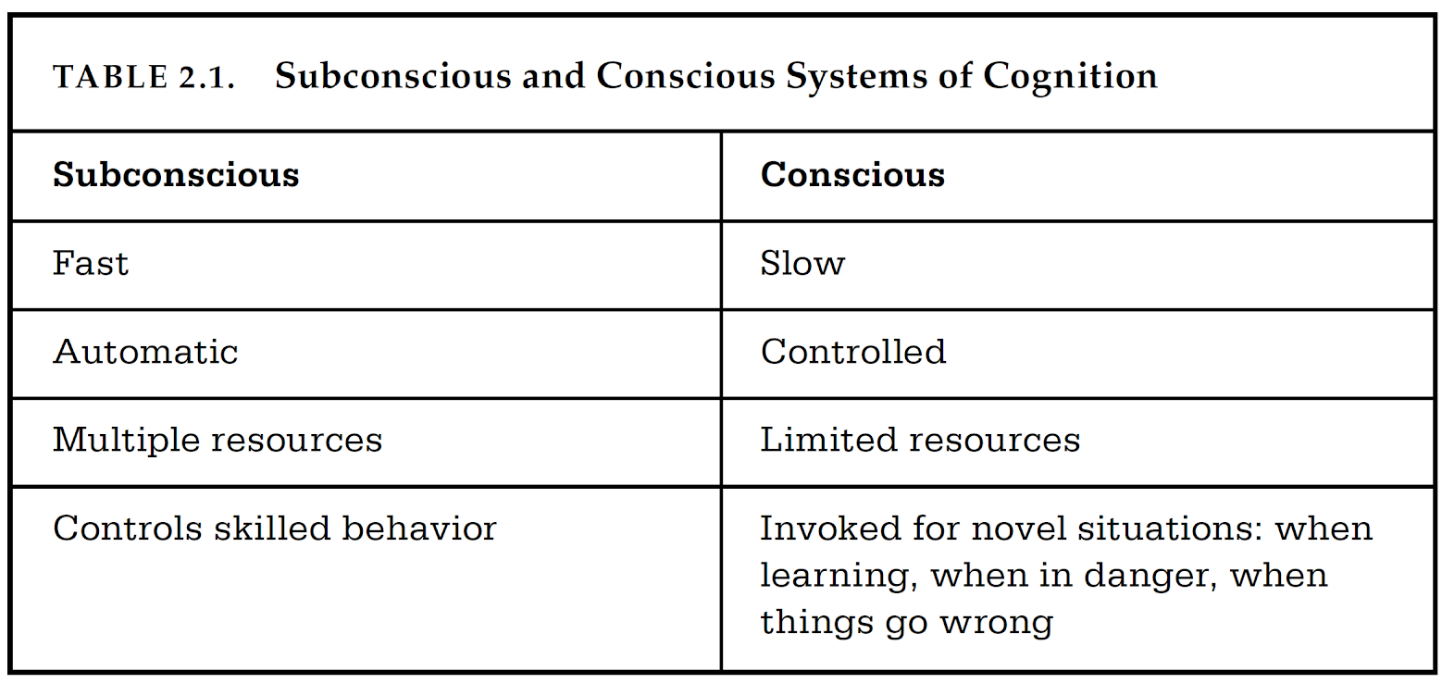
\includegraphics[scale=0.27]{immagini/subconscio-conscio.png}
\end{figure}

Un altro elemento determinante per il passaggio da un pensiero subconscio a uno conscio è lo stato emozionale.

\begin{figure}[!h]
	\centering
	\includegraphics[scale=0.75]{"immagini/Livelli di Processing"}
	\caption{Livelli di processing.}
\end{figure}

La divisione in conscio e subconscio può essere ulteriormente affinata andando a dividere il modo in cui il cervello fa processing in tre livelli
procedurali: viscerale (o rettiliano), comportamentale e riflessivo.

\begin{itemize}
	\itemsep-0.3em
	\item \textbf{Livello viscerale}: è il livello più elementare, permette di rispondere prontamente in maniera subconscia, senza consapevolezza o
	controllo cosciente.
	\item \textbf{Livello comportamentale}: è la sede delle abilità apprese durante circostanze più o meno simili a quelle attuali. Durante l'esecuzione,
	il livello comportamentale è guidato dalle aspettative, e durante l'attesa di conferma di tali aspettative è invece guidato dalle emozioni. Il livello
	comportamentale stabilisce in che modo si compie una determinata azione e in che modo si interpreta un determinato feedback.
	\item \textbf{Livello riflessivo}: è il livello della cognizione conscia, è qui che si sviluppa la comprensione profonda e hanno luogo il ragionamento
	e i processi decisionali. Qui fanno capo i livelli più alti di emotività: soddisfazione e orgoglio, ma anche frustrazione e senso di colpa.
\end{itemize}

\textbf{Veicolare informazioni all'utente mentre egli si trova nel livello riflessivo è estremamente efficace}. Al livello riflessivo il suo pensiero
è conscio e le emozioni che egli produce sono le più durature.

Gli stimoli riflessivi sono parte integrante del ricordo degli eventi, è importante quindi creare nell'utente ricordi positivi mentre egli è in questo
stadio dell'azione, perché tali ricordi sono i più duraturi.

Inoltre è la riflessione, intesa come pensiero cosciente, che induce a consigliare un prodotto e raccomandarne l'uso o magari a sconsigliarlo.

I tre livelli di elaborazione contribuiscono tutti insieme a determinare lo stato emotivo e cognitivo dell'utente. Funzioni riflessive di alto livello
possono mettere in moto emozioni più elementari e  queste, a loro volta, possono stimolare attività cognitive di tipo riflessivo. %How do people do things
\chapter{Errore Umano}

La maggior parte degli incidenti industriali è causata da errore umano:
le stime si aggirano tra il 75\% e il 95\% del totale.

\vspace{\baselineskip}
\textit{Come è possibile che tante persone siano così incompetenti?}
\vspace{\baselineskip}

La risposta è semplice! Non lo sono, il problema è nella mal progettazione e nel cattivo design.

Si continuano a produrre dispositivi e software che richiedono, a chi li usa, di mantenere per ore un'attenzione ed una vigilanza
complete, oppure di memorizzare procedure arcaiche, confuse e usate di rado, magari anche una sola volta nella vita. Si costringono
le persone a stare in un ambiente monotono senza nulla da fare per ore e ore, salvo dovere improvvisamente rispondere con rapidità e
precisione. Le si sottopone ad un ambiente di lavoro complesso e sovraccarico, dove sono continuamente interrotte durante l'esecuzione
di compiti simultanei. L'\textbf{interruzione è una delle cause che più frequentemente portano all'errore umano}.

Uno dei più grandi \textbf{problemi} è l'\textbf{atteggiamento delle persone verso gli errori} commessi. Quando un errore causa perdite economiche o,
peggio ancora, danni alle persone, si istituisce una speciale commissione d'inchiesta, che quasi immancabilmente trova i colpevoli.

Il passo successivo è punirli con multe, il licenziamento o addirittura il carcere. Essi vengono incolpati e puniti o, nella migliore delle ipotesi,
incolpati e riaddestrati. Tutto questo però non risolve il problema: lo \textbf{stesso errore continuerà a presentarsi}.  Per evitare di incorrere
nuovamente nell'errore, quando esso viene commesso, è bene  studiarne le cause, per poi ridisegnare il prodotto o le procedure in modo che esso non
si ripeta o, se dovesse ripetersi, che i danni siano ridotti al minimo.

\section{Root Cause Analysis}
La \textbf{Root Cause Analysis} consiste nell'indagare l'incidente finché non si trova la singola causa che ne è l'origine. Ovvero il momento nel tempo
quando effettivamente qualcuno ha preso decisioni o eseguito azioni sbagliate e,
una volta fatto ciò, accertare da cosa è derivato lo sbaglio. Purtroppo, troppo spesso, il processo si ferma non appena si scopre che una persona ha agito
in maniera impropria, additandola come \textit{colpevole}.

Cercare di trovare la causa di un incidente suona bene, ma ha due difetti.

\begin{itemize}
	\itemsep-0.3em
	\item La maggior parte degli incidenti \textbf{non ha una sola causa}. Da qui il \textbf{modello a groviera degli incidenti} di James Reason.
	\item Solitamente l'analisi delle cause profonde si ferma non appena trovato un errore umano.
\end{itemize}

\begin{figure}[!ht]
	\centering
	\includegraphics[scale=0.55]{immagini/Groviera.png}
	\caption{Modello a groviera.}
\end{figure}

Se una macchina smette di funzionare per un guasto o un malfunzionamento si cerca di capire come mai si è rotta o cosa l'ha portata a guastarsi. È
opportuno fare lo stesso quando si scopre un errore umano: \textbf{individuarne le cause}.

Quando durante l'analisi delle cause profonde si incontra, nella concatenazione di cause ed effetti, un errore umano, \textbf{il lavoro è appena
cominciato}: bisogna capire \textbf{perché} l'errore \textbf{è accaduto e cosa si può fare per prevenirlo}.

\section{I cinque perchè}

L'analisi delle cause profonde mira a determinare la causa \textbf{prima di un evento}, non la causa immediata.

In Giappone da tempo si usa a questo scopo una procedura detta \textit{"dei \textbf{cinque perché}"} ideata da Sakichi Toyota e impiegata dalla Toyota
nell'ambito del sistema di controllo qualità dei suoi prodotti.

Fondamentalmente quindi quando si cerca la ragione di un evento non ci si deve fermare dopo averne trovata solo una, ma bisogna continuare ad indagare
fino a che non si trovano le \textbf{vere cause di fondo}.

Va ripetuta davvero cinque volte?

No, ma chiamarla \textit{procedura dei cinque perché} sottolinea la necessità di proseguire anche dopo aver trovano una causa apparente.

Vediamo un esempio: \textbf{il veicolo non si accende}.

\begin{itemize}
	\itemsep-0.3em
	\item \textbf{Perché?} La batteria è morta.
	\item \textbf{Perché?} L'alimentatore non funziona.
	\item \textbf{Perché?} La cinghia dell'alternatore non funziona.
	\item \textbf{Perché?} La cinghia dell'alternatore era ben oltre il suo tempo di servizio e non è stata sostituita.
	\item \textbf{Perché?} Il veicolo non è stato mantenuto secondo le tempistiche raccomandate.
\end{itemize}

Quando le persone sbagliano, bisogna \textbf{cambiare il sistema} in modo da evitare l'errore
e, se non è possibile eliminarlo del tutto, almeno fare in modo di ridurne gli effetti.

Se il sistema lascia sbagliare gli utenti è \textbf{mal progettato}, se il sistema induce all'errore, allora è \textbf{progettato malissimo}.

\vspace{\baselineskip}
\textit{Perchè le persone sbagliano?}
\vspace{\baselineskip}

Perchè il design si concentra sulle esigenze del sistema e delle macchine, non su quelle degli utenti. Le macchine hanno bisogno in genere di
comandi precisi, obbligando l'operatore a introdurre esatte informazioni numeriche. Gli esseri umani non sono adatti ad esercitare grande precisione
e commettono spesso errori quando devono digitare lunghe sequenze di numeri o lettere.

Gli umani sono creativi, curiosi, costruttivi, particolarmente bravi nel creare modi nuovi di fare le cose e nel cogliere nuove opportunità. Compiti
monotoni, ripetitivi e precisi contraddicono tali qualità e vi entrano in conflitto.

\section{Definizione di errore}
Si definisce \textbf{errore umano} ogni deviazione dal comportamento \textit{appropriato}. Il termine appropriato è da prendere con le pinze, perché
in molte circostanze si scopre quale fosse il comportamento giusto solo successivamente.

Generalmente comunque si chiama \textit{errore} ogni comportamento che si discosta da quello generalmente accettato come giusto o adeguato.
\textbf{Errore} è il termine generale per tutte le situazioni sbagliate. È possibile dividere gli errori in \textbf{due} classi:

\begin{itemize}
	\item \textbf{Lapsus o Slips}: si ha un lapsus quando s'intende eseguire un'azione e si finisce per eseguirne un'altra. Nel caso del lapsus, l'azione
	eseguita non è quella voluta. Ci sono \textbf{due tipi principali di lapsus}:
	\vspace{-3.5mm}
	\begin{itemize}
		\itemsep-0.3em
		\item \textbf{di azione}: si esegue una azione sbagliata. Per esempio, si versa il latte nel caffé e si mette la tazza in frigo.
		\item \textbf{di memoria}: si dimentica di eseguire una azione o di valutarne i risultati. Per esempio, si dimentica il fornello acceso
		dopo aver terminato la cottura.
	\end{itemize}
	\textbf{I lapsus si hanno nelle fasi attuative e percettive dell'azione}.
	\item \textbf{Mistakes}: si ha un mistake quando è sbagliato il goal o lo scopo: da quel momento in poi le azioni, anche
	se eseguite a puntino, fanno parte dell'errore essendo di per sé inappropriate, in quanto parte di un progetto sbagliato. In questo tipo di errore
	l'azione è corretta ma l'intenzione no.
	I mistakes si suddividono in:
	\vspace{-3.5mm}
	\begin{itemize}
		\itemsep-0.3em
		\item \textbf{rule-based}: la diagnosi della situazione è giusta, ma poi viene scelto un corso d'azione sbagliato, seguendo una regola
		operativa errata. Per esempio, un meccanico diagnostica un difetto nella batteria di una macchina, decide di non sostituire la batteria perché
		funziona al 50\% delle prestazioni attese.
		\item \textbf{knowledge-based}: la diagnosi della situazione è sbagliata. Per esempio, il peso del carburante viene misurato in libbre anziché
		in chilogrammi.
		\item \textbf{memory-lapse}: un passaggio viene dimenticato nel momento in cui si fissano gli obiettivi o si esegue una procedura o se ne
		valutano i risultati. Per esempio, un meccanico fallisce nella gestione di un errore perché salta un passaggio.
	\end{itemize}
	\textbf{I mistakes si hanno nelle fasi di pianificazione e valutazione dell'azione}.
\end{itemize}

\begin{figure}[h!]
	\begin{subfigure}{0.49 \linewidth} \centering
			\includegraphics[scale=0.215]{immagini/Errors.png}
	\end{subfigure}
	\begin{subfigure}{0.49 \linewidth} \centering
			\includegraphics[scale=0.32]{immagini/Errors1.png}
	\end{subfigure}
\end{figure}


\section{Prevenzione dell'errore}

\begin{flushleft}
	\textit{Non dovrebbe essere possibile che un semplice errore provochi un danno diffuso.}
\end{flushleft}

Ecco che cosa dovrebbe essere fatto in fase di prevenzione:

\begin{itemize}
	\itemsep-0.3em
	\item \textbf{Comprendere le cause dell'errore} per minimizzarne il ripresentarsi.
	\item Effettuare \textbf{controlli di sensibilità}, ovvero, chiedersi se le azioni superano il \textit{test del buon senso}.
	\item Rendere possibile \textbf{annullare le azioni} (undo) o rendere più difficile fare ciò che non può essere annullato (per esempio con uso di locks).
	\item \textbf{Rendere} più \textbf{semplice la scoperta e la comprensione degli errori} e semplificarne la risoluzione.
	\item Non trattare l'azione come errore, piuttosto \textbf{aiutare l'utente a compiere correttamente l'azione}.
\end{itemize}

I \textbf{novizi}, gli utenti base, coloro meno esperti del sistema cadono in \textbf{mistakes} poiché non hanno una base di
conoscenza adeguata e sufficientemente strutturata, viceversa, gli \textbf{utenti esperti} che usano il software o il sistema tutti i giorni e
che lo conoscono bene commettono più errori di tipo \textbf{lapsus} poiché tendono ad eseguire i compiti in maniera automatica, quasi istintiva,
affidandosi al controllo subconscio, mentre un
principiante è costretto a fare molta attenzione, cosicché incorre meno nei lapsus.

I \textbf{mistakes} nascono dalla scelta di scopi e piani d'azione inadeguati, oppure, in sede di valutazione, dal confronto errato tra
risultati e scopi. In altre parole dipendono da \textbf{informazioni ambigue o poco chiare sullo stato attuale del sistema e dalla mancanza di un
buon modello concettuale}.

Si esamineranno adesso quali possono essere le cause di errore e come è possibile prevenirle.

Le \textbf{interruzioni} sono una delle più grandi cause di errore, \textbf{soprattutto i lapsus}. Quando un'attività viene interrotta da qualche
evento, il costo in attenzione è molto maggiore della perdita di tempo causata dell'interruzione. Per riprendere il lavoro è necessario ricordare
precisamente il precedente stato dell'attività: quale era l'obiettivo, a che punto del ciclo dell'azione si era rimasti e quale era lo stato del sistema.

La maggior parte dei sistemi rende difficile la ripresa di un azione a seguito di un'interruzione. Tuttavia riducendo i passaggi dell'azione è possibile
diminuire il costo d'attenzione necessario per riprendere la concentrazione dopo esser stati interrotti.

Un'altra causa di errore sono i \textbf{feedback errati}: avvisi fastidiosi o non necessari che si presentano spesso durante l'uso di un sistema. Spesso
vengono silenziati, disattivati o ignorati, \textbf{facendo perdere di significato anche quelli utili per il raggiungimento dello scopo}.

Se si usano i feedback per segnalare errori ed essi sono stati disattivati dall'utente, egli cadrà in errore non conoscendone nemmeno il motivo.
\textbf{Avvisi e metodi di sicurezza vanno usati con cura e intelligenza}.

Un numero sempre maggiore di macchine e sistemi offrono informazioni attraverso l'uso di interfacce vocali , ma come tutti gli approcci anche questo
ha dei pro e dei contro. Da una parte consente di fornire informazioni precise, specialmente quando
l'attenzione visiva è diretta da qualche altra parte, ma se l'ambiente è rumoroso o se ci sono diversi avvisi vocali contemporaneamente, tali avvisi
possono non essere compresi o risultare addirittura fastidiosi.

\pagebreak

\begin{figure}[!h]
	\centering
	\includegraphics[scale=0.6]{immagini/Damn.png}
\end{figure}

Per prevenire errori è possibile quindi utilizzare:
\begin{itemize}
	\itemsep-0.3em
	\item \textbf{Constraints}: aggiungendo vincoli alle azioni. I sistemi elettronici hanno un'ampia selezione di metodi che possono essere usati per
	ridurre l'errore. Uno di questi può essere \textbf{segregare i controlli}, cosicché controlli confondibili tra loro vengano piazzati lontani l'uno
	dall'altro. Un altro è di \textbf{separare i moduli}, cosicché qualsiasi controllo non direttamente rilevante all'operazione corrente non sia visibile
	a schermo ma richieda uno sforzo extra per essere raggiunto.
	\item \textbf{Undo}: comando che annulla le operazioni effettuate dal precedente. I sistemi migliori hanno \textbf{più livelli di undoing} in modo
	tale da annullare intere sequenze di azioni.
	\item \textbf{Messaggi d'errore e di conferma}: molti sistemi cercano di prevenire l'errore chiedendo conferma prima di eseguire un comando,
	specialmente quando l'azione distruggerà qualcosa di importante. Tuttavia queste richieste sono spesso mal temporeggiate, perché \textbf{dopo aver
	richiesto un'operazione le persone sono solitamente certe di volerla compiere}. Un controllo migliore sarebbe visualizzare sia l'azione da compiere
	che l'oggetto interessato, con l'opzione annulla o prosegui.\textbf{ I messaggi di avviso sono sorprendentemente inefficaci contro gli errori}.

	\item  \textbf{Controlli di Sensibilità}: i sistemi elettronici presentano il vantaggio di poter controllare che l'operazione richiesta sia
	\textbf{sensibile} o \textbf{ragionevole}. Ad esempio verificare che l'importo indicato sia giusto, magari esponendo un avviso in caso di numeri
	eccessivamente grandi.
\end{itemize}

In estrema sintesi e ricollegandosi all'esempio della groviera, per ridurre gli errori si hanno le seguenti possibilità:

\begin{figure}[!h]
	\centering
	\includegraphics[scale=0.5]{immagini/Groviera.png}
\end{figure}

\begin{itemize}
	\item \textbf{Aumentare il numero di controlli} (le fette).
	\item \textbf{Migliorare il modello concettuale dell'utente} (ridurre il numero di buchi, o rendere più piccoli i buchi esistenti, magari con un
	modello concettuale minimale e dei constraints).
	\item \textbf{Allertare l'operatore umano quando diversi buchi si allineano}.
\end{itemize} %errore
\chapter{Le interfacce utente}

Un'interfaccia è qualcosa che sta fra due facce. E' il punto di contatto fra due sistemi che tentano di comunicare. L'interfaccia serve quindi per
comunicare. Un'interfaccia può essere fisica (pulsanti), grafica (immagini a monitor) o di altre forme come per esempio un interprete, un traduttore
simultaneo o un mediatore culturale. 

Le interfacce possono far comunicare due macchine fra loro come nel caso del processore che tramite l'interfaccia USB scambia dati con la stampante.
Oppure possono far comunicare l’uomo con la macchina, come il cruscotto di un’auto, i cursori di un amplificatore, il rubinetto del lavandino, il
manubrio e i pedali della bicicletta.

Un'interfaccia utente è quindi sempre composta da due parti. Una di queste parti appartiene ad una persona l'altra ad uno strumento. Lo strumento è
ciò che compie l'azione, l’interfaccia è ciò che serve per permettere all'utente di guidare lo strumento nell'esecuzione dell'azione. Per esempio,
in un coltello la lama è lo strumento (che compie l'azione del tagliare), il manico è l’interfaccia che consente all'uomo di usare la lama senza
tagliarsi e quindi di guidare lo strumento in maniera soddisfacente. 

\begin{figure}[!h]
	\centering
	\includegraphics[scale=0.8]{immagini/interfaccia.png}
	\caption{Il manico è un esempio di interfaccia.}
\end{figure}


Quando parliamo di \textbf{User Interface o UI}, in italiano Interfaccia Utente, parliamo quindi dello spazio (non necessariamente fisico, il dominio
di una interazione ha una dimensionalità pari a quella dei nostri sensi) di un sistema dove avviene l'interazione fra uomo-macchina. Tipicamente,
si parla di UI in ambito informatico e tecnologico e quindi le interfacce utente sono comunemente identificate come sistemi atti a mettere in
comunicazione l'uomo con computer, sistemi informatici e oggetti intelligenti.

\vspace{\baselineskip}
\textit{User interfaces are a mapping from the sensory, cognitive, and social human world to these collections of functions exposed by a computer
program.}

[Amy J. Ko]
\vspace{\baselineskip}

L'obiettivo primario dell'interazione fra uomo e macchina è quello di consentire all'utente di controllare e far funzionare la macchina in modo efficace.
L'interfaccia deve quindi essere progettata per semplificare l'interazione fra l'uomo e la macchina rendendo così l'esperienza d'uso piacevole e
prolifica. L'interazione fra uomo e macchina deve sempre essere facile, efficiente e divertente così da massimizzare la User Experience del prodotto.

E' importante ricordare che l'uomo si è evoluto grazie alla sua capacità di adattamento che ha la sua massima espressione nel libero arbitrio e nella
capacità di prendere decisioni non necessariamente basate sulla logica ma piuttosto sulle sensazioni e intuizioni. Viceversa le macchine hanno un
comportamento puramente deterministico e pertanto non hanno nessuna capacità di adattamento. L'interfacci uomo macchina va quindi ad avere un ruolo
fondamentale nell'interazione fra le parti dal momento che abilita la comunicazione fra due realtà aventi principi e modalità di "funzionamento"
diametralmente opposte.

Un'interfaccia ben progettata consente all'utente di controllare l'apparato richiedendo uno sforzo fisico e cognitivo minimo. La buona interfaccia
massimizza inoltre la quantità di informazioni utili trasferite all'utente durante l'interazione evitando un sovraccarico informativo che provocherebbe
nell'utente confusione e quindi frustrazione.

\begin{figure}[!h]
	\centering
	\includegraphics[width=0.9\textwidth]{immagini/tesla.jpg}
	\caption{Cruscotto della Tesla model S (\href{https://pinxcars.com/2013-tesla-model-s-cockpit/}{\underline{Fonte}}.)}
\end{figure}

Per questo motivo, la progettazione di un'interfaccia è per definizione un'attività interdisciplinare che va oltre la programmazione grafica e
abbraccia la psicologia, le neuroscienze, il design e la fisica.

Le interfacce sono organizzabili secondo livelli. L' \textbf{HID o Human Interface Device} è la periferica grazie al quale l'utente interagisce con
il sistema; come ad esempio mouse, monitor, gamepad, ecc.. Lo \textbf{HMI o Human Machine Interface} è invece un concetto che astrae dall' HID.
Con HMI, si intende infatti, tutto il sistema di interazione uomo macchina che usa l'HID come elemento di contatto fisico con l'utente. Nel computer
per esempio, la HMI è il sistema mouse+cursore+finestre. Il mouse e il monitor sono HID.

Quando la macchina in questione è un computer, HMI diviene \textbf{HCI o Human Computer Interface}.

\section{Classificazione delle interfacce}
Le interfacce utente sono tipicamente organizzate sulla base dei sensi che utilizzano per stabilire l'interazione fra umano e macchina. Gli umani
possiedono cinque sensi (tatto, vista, udito, olfatto e gusto). Questo porta ad identificare cinque categorie di interfacce possibili, più una sesta
che è legata al cosidetto senso dell'equilibrio (balance in inglese) che però non è considerato un senso vero e proprio nella fisiologia umana.

Possiamo quindi organizzare le interfacce in 6 categorie:
\begin{itemize}
	\itemsep-0.3em
	\item \textbf{Tactile UI} (touch, tatto);
	\item \textbf{Visual UI} (sight, vista);
	\item \textbf{Auditory UI} (sound, udito);
	\item \textbf{Olfactory UI} (smell, olfatto);
	\item \textbf{Gustatory UI} (taste, gusto);
	\item \textbf{equilibrial UI} (balance, equilibrio).
\end{itemize}

La maggior parte delle interfacce utente utilizza però più di un senso umano per stabilire il collegamento. Le interfacce che usano più di un senso
sono dette \textbf{CUI o Composite User Interface}. Le più comuni e note CUI sono chiaramente le famose \textbf{GUI o Graphical User Interface},
le quali sono composte da interfacce grafiche (visual) e tattili (tactile). 

Se ad una GUI andiamo ad aggiungere anche il suono otteniamo una \textbf{MUI o Multimedia User Interface}.

Quindi quando ci si riferisce all'interfaccia di una app con il termine GUI spesso compiamo un errore perchè ormai la maggior parte dei dispositivi
informatici ha anche una sorgente sonora che è utilizzata durante l'interazione (feedback audio del touch sullo schermo, per esempio) e quindi ci
troviamo di fronte ad una MUI e non ad una GUI.


È bene sottolineare che \textbf{estendere le interfacce con più canali (sensi) non è sempre una buona idea}.
\begin{figure}[!h]
	\centering
	\includegraphics[scale=0.85]{immagini/flora_video.png}
	\caption{Esempio: video di Facebook (\href{https://www.facebook.com/Lastknight/posts/10158944882367053}{\underline{Fonte}}).}
\end{figure}

Prendiamo ad esempio i video di
Facebook, i video vengono riprodotti di default con l'audio disattivato per aumentare l'usabilità del sistema.
Gli ingegneri di Facebook si sono accorti infatti che la maggioranza delle persone che visualizzando i video, mutavano immediatamente il suono per
varie ragioni (e.g. privacy o utilizzo di Facebook in momenti non opportuni), quindi hanno reso questa opzione di default. Ovviamente se ragionassimo
in termini di capacità e possibilità dell'interfaccia sembrerebbe assurdo bloccare di default l'utilizzo di un canale.
Questo processo di analisi ha portato poi a far evolvere il mondo dei video online inserendo di default i sottotitoli. Siamo quindi in una situazione in
cui per aumentare l'usabilità del sistema se ne riducono le funzionalità (di default).

%Questo, oltre ad essere un ottimo esempio di MUI riprogettata in GUI, è anche un esempio di tecnica ideata per gli utenti disabili e riusata per
%far fruire il prodotto a quelle personas che lo utilizzano in momenti in cui non possono usufruire dell'audio.


\section{Categorizzare le CUI}
Le CUI possono essere categorizzare in tre diverse macrocategorie:

\begin{itemize}
	\itemsep-0.3em
	\item \textbf{Standard}: usano dispositivi standard come tastiere, mouse e monitor
	\item \textbf{Virtual}: Bloccano all'utente l'interazione con il mondo reale e creano un mondo virtuale che funge da interfaccia fra l'utente e
	la macchina.
	\item \textbf{Augmented}: Non bloccano all'utente la percezione del mondo reale ma la vanno ad arricchire. L'interfaccia è quindi un mix di
	contenuti reali e virtuali che vanno ad arricchire la realtà \textbf{espandendola}.
\end{itemize}

\begin{figure}[!h]
	\centering
	\includegraphics[width=\textwidth]{immagini/standard-virtual-interfaces.png}
	\caption{Tipi di interfaccia.}
\end{figure}

Le CUI possono essere anche \textbf{classificate tramite il numero di sensi che utilizzano}. Ad esempio, lo \textit{Smell-O-Vision} è una CUI
standard 3S, cioè è una normale interfaccia di tipo standard che nell'utilizzo coinvolge 3 sensi dell'utente (Visione, Udito e Olfatto). Se si
aggiungesse un quarto senso (per esempio le poltrone mobili dei cinema 4D) diventerebbe 4S.

Quando un'interfaccia utente interagisce con tutti i sensi umani viene chiamata \textbf{Qualia Interface} (il termine ``qualia" deriva
dalla \href{https://it.wikipedia.org/wiki/Qualia}{\underline{teoria filosofica dei qualia}}).

\begin{figure}[!h]
	\centering
	\includegraphics[scale=0.2]{immagini/react.jpg}
	\caption{Esempio di interfaccia aumentata 3S: Microsoft Reactable.}
\end{figure}

\section{Human Interface Devices}

Un ``human interface device" è un dispositivo informatico usato da umani e, tipicamente, prende input da umani; col termine HID si intendono sia i
\textbf{dispositivi fisici} sia il \textbf{protocollo USB-HID}.

\subsection*{Protocollo HID}

Il termine HID è stato coniato da Microsoft per permettere l'innovazione nell'ambito dei dispositivi di input e per semplificare il processo di
installazione di questi dispositivi; prima dell'introduzione dello standard, questi seguivano protocolli che dipendevano dal loro tipo
(mouse, tastiere, joystick etc.): nel caso di nuovi dispositivi, le opzioni erano adeguarsi a un protocollo già esistente o sviluppare
nuovi driver specifici. Invece, i dispositivi HID spediscono pacchetti che ne descrivono il tipo e che contengono dati di svariati tipi e formati.

Un singolo driver HID procede col parsing del pacchetto di dati e permette l'associazione dinamica di dati I/O con le funzionalità del sistema: è
possibile mandare dati come dispositivo standard e, per esempio, lasciare al sistema operativo il compito di decidere come utilizzarli. Il protocollo
ha dei limiti, ma i sistemi operativi moderni riconoscono dispositivi USB HID standard (mouse, tastiera) senza bisogno di driver specifici.

Nel protocollo HID si distinguono due entità:
\begin{itemize}
	\itemsep-0.3em
	\item \textbf{device}: interagisce direttamente con l'umano.
	\item \textbf{host}: comunica col device e riceve dati sulla base delle azioni eseguite dall'umano; i dati in output vanno dall'host al
	device all'umano.
\end{itemize}

Inoltre, il protocollo ha reso molto semplice la costruzione di nuovi dispositivi introducendo il concetto di \textbf{HID descriptor}:
\textbf{è un pacchetto standard che definisce la categoria di appartenenza e la struttura di dato del device} (NON ha bisogno di essere generato
dal dispositivo, può essere hard coded) e che viene inviato non appena il device viene collegato all'host.
Tipicamente, il device salva sulla ROM l'HID descriptor e non ha bisogno di capirlo; infatti, alcuni mouse e tastiere in commercio sono implementate
usando una CPU a 8-bit.

Il ruolo dell'host è più complesso poich\'e ha bisogno di ricevere l'HID descriptor dal device e farne il parsing prima di poter comunicare con questo:
ha bisogno della potenza computazionale necessaria per l'interpretazione del pacchetto.
Essendo chiaro che non tutti gli host potrebbero essere capaci di interpretare l'HID descriptor, HID descrive anche il ``boot protocol": prevedendo
pacchetti di formato predefinito, sono supportati solo alcuni device specifici (solo tastiera e mouse) con alcune feature specifiche.

HID è stato esteso a una serie di protocolli, si riportano alcuni esempi:
\begin{itemize}
	\itemsep-0.3em 
	\item \textbf{Bluetooth HID}: usato per mouse e tastiere connesse via Bluetooth.
	\item \textbf{Serial HID}: usato per telecomandi su Windows Media Center.
	\item \textbf{ZigBee input device}: ZigBee (RF4CE) supporta dispositivi HID attraverso il profilo ZigBee input device.
	\item \textbf{HID over I²C}: usato per dispositivi embedded su Microsoft Windows 8.
	\item \textbf{HOGP} (HID over GATT): usato per dispositivi HID connessi attraverso BLE.
\end{itemize}

\pagebreak
\subsection*{Periferiche HID}

Le periferiche HID sono organizzate in due categorie:
\begin{itemize}
	\itemsep-0.3em
	\item \textbf{di input}: basati su sensori, converte la realtà fisica in segnale elettrici. Un esempio di sensore è un microfono.
	\item \textbf{di output}: basati su attuatori, converte segnali elettrici in perturbazioni nel mondo. Un esempio di attuatore è un altoparlante.
\end{itemize}

Dispositivi di input e di output venivano tradizionalmente divisi in classi sulla base del tipo di input/output usato dall'HID, al giorno d'oggi questa
classificazione tende a decadere poich\'e la maggior parte dei dispositivi moderni usano più tecnologie; di seguito, le classi:
\begin{itemize}
	\itemsep-0.3em
	\item \textbf{testi e caratteri};
	\item \textbf{posizioni};
	\item \textbf{suoni};
	\item \textbf{immagini};
	\item \textbf{parametri ambientali};
	\item \textbf{posizione};
	\item \textbf{parametri fisiologici e biologici}.
\end{itemize}

\subsubsection*{HID testi e caratteri}
L'HID della classe testi e caratteri più comune è la \textbf{tastiera}.
Tre layout sono da prendere in considerazione per le tastiere:
\begin{itemize}
	\itemsep-0.3em 
	\item \textbf{layout fisico}: corrisponde al posizionamento dei tasti sulla tastiera. \`E normato.
	\item \textbf{layout visuale}: corrisponde all'arrangiamento dei simboli che appaiono sui tasti. Ad esempio, qwerty, azerty etc.
	\item \textbf{layout funzionale}: corrisponde all'associazione tasto-significato all'interno di un software. Ad esempio, quando si apre YouTube
	viene messo a disposizione un layout funzionale in cui alla barra spaziatrice si fa corrispondere riproduzione e pausa.
\end{itemize}

\begin{figure}[!h]
	\centering
	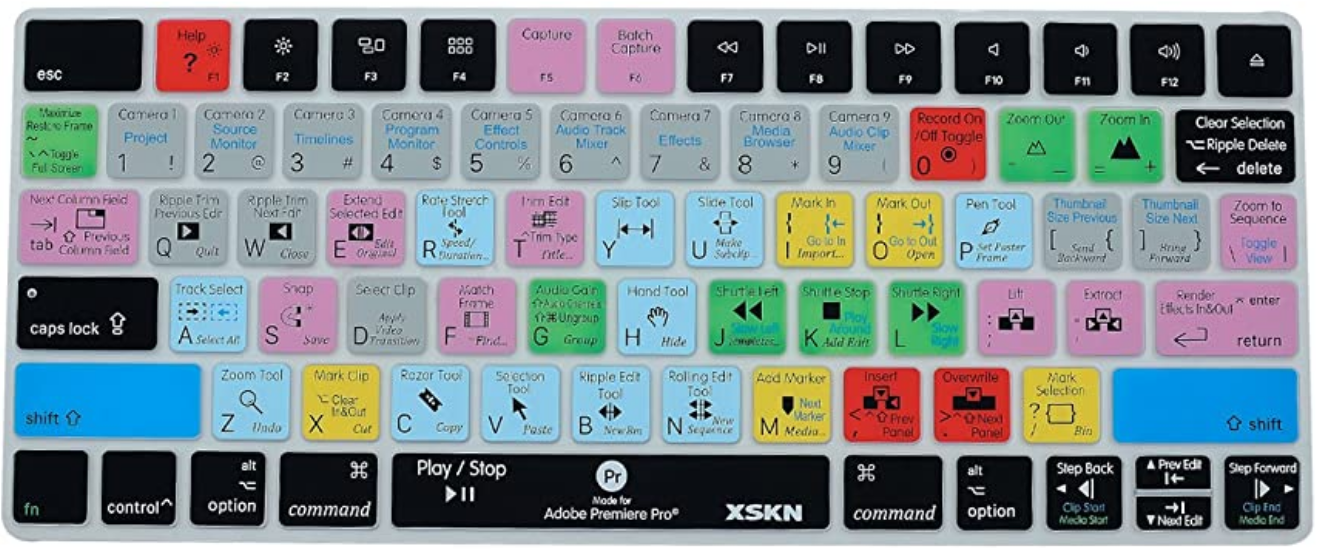
\includegraphics[scale=0.25]{immagini/adobe-layout-funzionale.png}
	\caption{Esempio di layout funzionale di una tastiera su Adobe Premiere Pro.}
\end{figure}

Esistono inoltre \textbf{tastiere multifunzione}, che estendono tastiere standard con altri tasti e mappature; necessitano di driver aggiuntivi a meno
che il produttore non le faccia apparire come una tastiera standard estesa e poi deleghi a un applicativo il compito di associare un layout funzionale
appropriato.

Un altro dispositivo HID testi e caratteri è il \textbf{lettore di codice a barre}: concretamente, è un serializzatore di caratteri. Un codice QR è un
\textbf{barcode} bidimensionale che usa quattro modalità di encoding per salvare i dati in modo efficiente.

I \textbf{tag RFID} sono formati da un transponditore radio (cioè un trasmettitore e un ricevitore radio); ne esistono di \textbf{passivi} (fanno
energy harvesting, prendono la potenza dall'onda elettromagnetica che impatta con l'antenna dell'host; l'antitaccheggio dei negozi usano un RFID passivo)
e di \textbf{attivi} (usano una batteria e si usano tipicamente per la geolocalizzazione).

\textbf{NOTA BENE}. RFID e NFC non sono la stessa cosa: NFC permette comunicazioni bidirezionali, non è per solo input.

\subsubsection*{Sistemi di puntamento}
Sono dispositivi di input che trasferiscono input di tipo spaziale verso un computer: i movimenti fisici dell'utente vengono replicati su uno schermo
attraverso movimenti di un puntatori e/o altri cambiamenti visivi.

Si definisce in merito la \textbf{legge di Fitt} per il calcolo del tempo di movimento MT: \( MT = a + b * ID = a + b * \log_2 \frac{2D}{W} \)

con \textbf{a} definito come il tempo (in secondi) necessario per iniziare o smettere di muoversi (si misura empiricamente per ciascun dispositivo),
\textbf{b} la velocit\`a del dispositivo (si misura empiricamente per ciascun dispositivo),
\textbf{D} la distanza dal punto iniziale al centro dell'obiettivo,
\textbf{W} la larghezza dell'obiettivo misurata lungo l'asse su cui ci si sta muovendo.

Si danno i seguenti criteri per la classificazione di dispositivi di puntamento:
\begin{itemize}
	\itemsep-0.3em
	\item sulla base del \textbf{tipo di input}:
	\vspace{-3mm}
	\begin{itemize}
		\itemsep-0.3em
		\item \textbf{diretto} se il puntatore si trova nella stessa posizione fisica che il device (ad esempio, il dito su un touch screen);
		\item \textbf{indiretto} quando traduce il movimento sullo schermo (ad esempio, il mouse o lo stilo di una tavoletta grafica).
	\end{itemize}
	\item sulla base del \textbf{modo in cui il movimento viene mappato} sull'interfaccia:
	\vspace{-3mm}
	\begin{itemize}
		\itemsep-0.3em
		\item \textbf{assoluto} quando il mapping tra lo spostamento nel mondo fisico viene replicato così com'è sul dispositivo;
		\item \textbf{relativo} altrimenti.
	\end{itemize}
	\item sulla base di \textbf{come} i dispositivi producano il segnale sulla base dello spostamento:
	\vspace{-3mm}
	\begin{itemize}
		\itemsep-0.3em
		\item \textbf{isotonico} (stesso tono), si può muovere nello spazio e misura lo spostamento;
		\item \textbf{isometrico} (stesso metro), è fisso e misura la forza che viene applicata;
		\item \textbf{elastico}, la forza applicata è proporzionale allo spostamento (ad esempio, il joystick a molla).
	\end{itemize}
	\item sulla base della \textbf{velocità con cui si fa avanzare il puntatore}:
	\vspace{-3mm}
	\begin{itemize}
		\itemsep-0.3em
		\item \textbf{position control}, si controlla la posizione (relativa o assoluta) del puntatore;
		\item \textbf{rate control}, si controlla la velocità e la direzione del puntatore (ad esempio, i joystick degli arcade games).
	\end{itemize}
\end{itemize} %Le interfacce utente
\chapter{UX Design}
\begin{flushleft}
	\textit{Quali processi e metodi utilizzare per portare avanti il progetto di un prodotto software?}
\end{flushleft}

In questo capitolo si analizzeranno diversi processi.
Essi non vanno identificati come fasi ben definite e statiche, da seguirsi una dietro l'altra, bensì come \textbf{fasi} \textbf{dinamiche} e
\textbf{alternabili}.

\section{Personas}
Identificato correttamente il problema mediante la \textbf{Task Analysis}, come si  possono creare elementi individuali? Come si identificano le
cosiddette \textbf{Personas}?

\begin{figure}[!h]
	\centering
	\includegraphics[scale=0.55]{immagini/Personas.png}
\end{figure}

Il primo passo da fare dopo la Task Analysys è \textbf{identificare le personas}.
Una \textbf{user persona} è l'\textbf{archetipo di uno dei possibili utenti}. Scrivere e
identificare le personas aiuta a colmare la distanza tra il cliente e l'azienda, in modo da capire cosa vuole e cosa si aspetta l'utente dal prodotto,
ma anche cosa gli crea frustrazione nell'usarlo.
Esistono molte \textbf{tecniche} atte a fare fare un'analisi degli utenti e che aiutano i progettisti a identificare e a scrivere le personas:

\begin{itemize}
	\itemsep-0.3em
	\item \textbf{Task Analysis}.
	\item \textbf{Feedback} tra i quali: analisi delle attività, interviste e focus groups.
	\item \textbf{Prototipazione}.
\end{itemize}

Sorge spontanea la domanda seguente: \textit{ma quante personas è bene definire}?
Per rispondere a questa domanda ci si basa sul \textbf{Principio di Pareto}:

\textit{Concentrarsi sul 20\% degli utenti che utilizzerà il prodotto per l'80\% dell'uso complessivo.}

\pagebreak

\section{Requirements}

Un \textbf{requirement} è un servizio o una caratteristica che soddisfa un bisogno di un utente.
I requirements possono essere funzioni, vincoli, regole aziendali o altri tipi di elementi di cui il prodotto deve essere dotato per soddisfare le
esigenze degli utenti. È quasi ovvio che trovare i \textbf{requirements corretti} risulta molto più \textbf{semplice} se in precedenza sono state
\textbf{individuate} e \textbf{descritte} le \textbf{personas}.

Infatti è controproducente scrivere anticipatamente i requirements,
è complesso se non impossibile descriverli tutti all'inizio di una fase di progettazione. Risulta più facile descrivere i requirements con l'avanzamento
del progetto, in modo da poter capire come modificare, eliminare o aggiungere i requirements giusti, tenendo in considerazione anche le personas a cui
è destinato il prodotto finale.

Il \textbf{requirements driven development} è un approccio complesso e oneroso e va in \textbf{contrasto} con il metodo \textbf{Agile} che richiede si
sia sempre pronti al cambiamento. Questo approccio così poco flessibile sta andando sempre meno di moda tuttavia è bene seguirlo una volta definiti i
requirements per quel 20\% di software che utilizzerà l'80\% delle personas.

Esistono \textbf{due tipi di requirements} per il mondo della UI:

\begin{itemize}
	\itemsep-0.3em
	\item \textbf{Funzionali}: descrivono quali funzionalità deve avere il software. Rispondono alla domanda: \textit{Cosa fa?}
	\item \textbf{Non funzionali}: specificano i tratti qualitativi del prodotto. Rispondono alla domanda: \textit{Come lo fa?} e descrivono inoltre
	attributi come sicurezza, affidabilità e manutenibilità.
\end{itemize}

\section{User Stories}
Dopo aver definito \textbf{personas} e \textbf{requirements}, il prossimo passo è la scrittura delle \textbf{User Stories}.

Una \textbf{user story} è una breve descrizione che identifica l'utente insieme al suo obiettivo e alle sue necessità, determina \textbf{chi è},
\textbf{di cosa ha bisogno e perché ne ha bisogno}. Tipicamente ci sono una o più user stories per ogni personas, ma \textbf{non il contrario}: avere
più personas per una user story significa aver descritto la medesima persona con termini differenti e quindi averne introdotta una ridondante. Se una
user story non copre tutte le sfaccettature della singola persona che dovrebbe descrivere è indizio del fatto che tale persona potrebbe essere
troppo \textbf{ampia}, ed è bene che venga suddivisa in più personas.

Una user story è un \textbf{requirement} espresso \textbf{dalla prospettiva del cliente}.

Con le user stories si ottengono due importanti risultati: si \textbf{migliorano le descrizioni delle personas}, migliorandone il dettaglio e
arricchendole con una narrativa, e si ha un elemento tangibile per valutare lo sviluppo del prodotto e fare il punto della situazione.
Esiste uno schema ben preciso per scrivere una user story:

\begin{center}
	\textbf{\large As a [role], I want [feature] because [reason]}.
\end{center}

Questo approccio permette di pensare a chi abbia bisogno di una certa funzionalità e per quale motivo (ne abbia bisogno); inoltre, ordinare i
bisogni delle varie personas e le personas per importanza permette di ordinare le user stories e, di conseguenza, i requirements.

\begin{flushleft}
	\textit{Chi scrive le user stories?}
\end{flushleft}

\textbf{Tutti}! È responsabilità del proprietario del prodotto assicurarsi che vengano scritte delle stories giuste e corrette, ma non significa che
le debba scrivere lui stesso. Nel corso di un buon progetto Agile ci si aspetta che ogni membro del team partecipi alla scrittura delle user stories
secondo un \textbf{metodo collaborativo}. \`E importante ricordare che chi scrive una user story è molto meno importante di chi è coinvolto nelle
discussioni su queste.

\begin{flushleft}
	\textit{A che livello è bene scriverle?}
\end{flushleft}

Uno dei grandi benefici delle user stories è che possono essere
scritte a \textbf{vari livelli di dettaglio}.

Possiamo avere user story di livello \textbf{epic}, ovvero in grado di coprire un grande quantità di funzionalità; tipicamente sono disutili, ma
possono diventare interessanti se spacchettate in user stories più piccole e, di conseguenza, più dettagliate. Una \textbf{user story epic} può
essere \textbf{divisa} in decine o centinaia di user stories più piccole.

I dettagli possono essere aggiunti sostanzialmente in due modi:
\begin{enumerate}
	\itemsep-0.3em
	\item Suddividendo una user story in user stories più piccole e quindi più dettagliate.
	\item Aggiungendo \textbf{condizioni di soddisfacimento dell'utente}, ovvero dettagli che contribuiscono al grado di soddisfacimento
	dell'utilizzatore del prodotto, suddividendole per ogni eventuale membro di soddisfacimento. Quest'ultima è una tecnica molto difficile da
	utilizzare nel mondo della progettazione software.
\end{enumerate}

\section{Scenarios}

Gli \textbf{scenarios} sono l'\textbf{evoluzione delle user stories}. Una user story sintetizza in brevi frasi cosa fa l'utente con il software e
quale bisogno deve soddisfare.

Lo \textbf{scenario estende la user story} andando a descrivere anche quali motivazioni hanno portato l'utente a usare il software e come si
comporterà nel suo utilizzo. Inoltre gli scopi o \textbf{goals} delle personas vengono \textbf{estesi} e descritti in maniera più ampia.

\begin{flushleft}
	\textit{Ma a cosa serve uno scenario?}
\end{flushleft}

Le \textbf{user stories} sono \textbf{sintetiche}, \textbf{brevi}, dicono cosa sviluppare e poco più, sono informative e comprensibili
\textbf{solo} agli \textbf{addetti al mestiere}. Gli \textbf{scenarios}, essendo più ricchi in dettaglio, sono più comprensibili agli
\textbf{stakeholders} (ossia alle persone interessate al prodotto), quindi sono \textbf{utili per comunicare e interloquire con persone fuori dal
team di sviluppo}. Servono soprattutto per allinearsi con le richieste del cliente ma sono  utili anche all'interno del team per allineare le idee.

Un buon scenario risponde alle \textbf{seguenti domande chiave}:

\begin{itemize}
	\itemsep-0.3em
	\item \textbf{Chi è l'utente?}
	\item \textbf{Quale è la motivazione che lo ha spinto ad usare il prodotto e cosa si aspetta da esso?}
	\item \textbf{Qual è il suo obiettivo?}
\end{itemize}

In alcuni casi uno scenario potrebbe includere anche aspetti circa \textit{come} fare le cose, ma ciò appartiene al mondo degli \textit{use cases}
che verranno analizzati successivamente. Per \textbf{definire gli scenarios}, è necessario \textbf{mapparli}. Bisogna partire \textbf{avendo già
definito le personas e le relative user stories}, e individuare per ogni persona un \textbf{key task} che essa deve svolgere. Si possono scrivere
gli scenarios racchiudendo una o più user stories relative alla persona ma tipicamente per ogni persona si descrive  almeno uno scenario.
È necessario \textbf{focalizzarsi sul key task} e quindi \textbf{contestualizzare} nel miglior modo possibile il goal dell'utente e come è
influenzato dal contesto in cui egli si trova.

Quindi grazie agli scenarios \textbf{possiamo determinare}:

\begin{itemize}
	\itemsep-0.3em
	\item I \textbf{punti più importanti} su cui concentrarsi durante il \textbf{processo di progettazione per l'UX}.
	\item Quali fasi del processo richiedono \textbf{ulteriore revisione e attenzione}.
	\item Le \textbf{principali esigenze e motivazioni dell'utente}.
\end{itemize}

Ci sono \textbf{tre metodi principali per scrivere gli scenarios}:

\begin{itemize}
	\itemsep-0.3em
	\item Piccoli \textbf{goal or task oriented scenarios}: sono brevi, quasi una semplice estensione della dialettica di una user story.
	\item \textbf{Elaborated Scenarios}: sono versione più elaborata e con molto più contesto.
	\item \textbf{Full Scale Task Scenarios}: sono talmente dettagliati che i singoli task delle attività sono praticamente scritti sotto forma di
	paragrafo. Sono da evitare poiché si rischia gli scenarios così ottenuti siano uguali agli use cases.
\end{itemize}

\section{Use Cases}

Gli use cases sono la naturale evoluzione degli scenarios.
\textbf{Consistono della completa narrativa di quali azioni l'utente compie per svolgere uno scenario}.

Ogni \textbf{caso d'uso} è una \textbf{serie di step monolitici}, è quindi una nuova task list prodotta dal processo di design per ampliare 
ulteriormente un concetto analizzato e descritto in precedenza mediante la task analysis. Uno \textbf{scenario} si concentra su una situazione che
coinvolge uno o più \textbf{attori}, mentre un \textbf{caso d'uso} è incentrato su una \textbf{persona}, come essa si comporta, che decisioni prende
e come interagisce con la nostra piattaforma o software. I casi d'uso aggiungono informazione perché aiutano a \textbf{spiegare come dovrebbero
comportarsi il sistema e il processo}, inoltre aiutano anche nella fase progettuale di brainstorming e danno un'idea su cosa potrebbe andare storto.
Forniscono inoltre un elenco di obiettivi che può essere utilizzato per stabilire e valutare la complessità del sistema. I casi d'uso sono
\textbf{diretti allo sviluppo}.

Con dei \textbf{casi d'uso ben fatti} si può passare direttamente all'\textbf{implementazione} poiché \textbf{delimitano precisamente cosa deve fare
il sistema e come si deve comportare nelle varie situazioni}.

In un caso d'uso sono \textbf{inclusi}:
\begin{itemize}
	\itemsep-0.3em
	\item \textbf{L'utente}.
	\item \textbf{Cosa vuole fare}.
	\item \textbf{Qual è il suo scopo o goal}.
	\item Gli \textbf{step necessari} per arrivare allo scopo.
	\item I \textbf{feedback} che il sistema restituisce durante i vari step.
	\item i \textbf{trigger} che causano l'avvio del caso d'uso.
	\item Il \textbf{basic flow}, ossia il caso d'uso in cui non avvengono errori di alcun tipo.
	\item \textbf{Alternative flow}, ossia il caso d'uso in cui si hanno eccezioni dovute a qualche parte del sistema malfunzionante.
\end{itemize}

\textbf{Non sono inclusi} in un caso d'uso:
\begin{itemize}
	\itemsep-0.3em
	\item Qualsiasi \textbf{dettaglio implementativo o di scelta tecnologica} che non sia un constraint o un requirement.
	\item \textbf{Dettagli} riguardanti l'interfaccia utente.
\end{itemize}

I passaggi da seguire per scrivere un caso d'uso sono:

\begin{enumerate}
	\itemsep-0.3em
	\item Identificare le \textbf{personas}.
	\item Sceglierne \textbf{una per caso d'uso}.
	\item Identificare i suoi \textbf{obiettivi}.
	\item Discernere i \textbf{task principali} da quelli \textbf{secondari}: applicare il principio di Pareto, quindi focalizzarsi sul basic path e
	non su casi particolari.
	\item Considerare le sequenze alternative.
	\item Cercare i punti in comune tra i vari casi d'uso e \textbf{accorparli}, riducendoli ove possibile.
	\item Ripetere il procedimento per tutti gli utenti.
\end{enumerate}

Questi passaggi, eseguiti correttamente, consentono di identificare informazioni chiave sugli utenti, utili a costruire prodotti che soddisferanno
tutte le possibili personas. \textbf{Ogni passo che ci avvicina all'utente è un passo verso la giusta direzione}.
\chapter{Metodi e Strumenti per l'Innovazione}

Introduciamo ora una serie di metodi di lavoro e strumenti nati per facilitare la progettazione e realizzazione di prodotti e sistemi innovativi. 

\begin{flushleft}
\textit{ \textbf{Innovazióne} s. f. [dal lat. tardo innovatio -onis]. L’atto, l’opera di innovare, cioè di introdurre nuovi sistemi, nuovi ordinamenti,
nuovi metodi di produzione. In senso concreto, ogni novità, mutamento, trasformazione che modifichi radicalmente o provochi comunque un efficace
svecchiamento in un ordinamento politico o sociale, in un metodo di produzione, in una tecnica, ecc. [Treccani]}
\end{flushleft}

Il concetto di innovazione è legato a quello di progresso tecnologico, ma non sono la stessa cosa: l'innovazione riguarda le applicazioni di una certa
tecnologia e non ha sempre bisogno di nuova tecnologia.
In innovazione, l'applicazione della filosofia HCD diventa di vitale importanza dal momento che un prodotto o servizio per essere innovativo deve
essere prima di tutto apprezzato dagli utenti e quindi utilizzato.

\textbf{Cosa vuol dire innovare? Esiste un solo modo di fare innovazione?}

\section{Disruptive Innovation}
\begin{flushleft}
	\textit{\textbf{People don’t want to buy a quarter-inch drill. They want a quarter-inch hole!} - Professor Theodore Levitt,
	Harvard Business School}
\end{flushleft}

La maggior parte dell'innovazione è fatta come miglioramento incrementale di prodotti o sistemi già esistenti. I nuovi condizionatori d'aria, per
esempio, hanno motori e gas più efficienti rispetto al passato ma il loro funzionamento è basato sul principio della macchina frigorifera che fu
proposto per la prima volta nel 1835.
Questo approccio all'innovazione fatta attraverso piccole migliorie apportate ad un sistema stabile è il più comune. Questo processo passo-passo è
molto affidabile, consente di raggiungere buoni risultati con investimenti tutto sommato contenuti e di mantenere invariata la struttura delle aziende
(produttori) e della società (consumatore). Questo processo di innovazione incrementale ha però bassissime probabilità di portare ad una modifica
sostanziale del prodotto/processo su cui è applicato.

L'\textbf{Innovazione Incrementale} (o \textbf{Sustaining Innovation}) punta infatti al mantenimento della competitività aziendale tramite un processo
passo-passo dove si fa un aggiornamento alla volta. Nel paradigma di innovazione incrementale la clientela di riferimento è stabile e definita e non
si punta solitamente ad espandere il business verso altre nicchie di clientela.

In generale però, quando si parla di innovazione, ci si aspetta di trovarsi davanti ad un prodotto o servizio che cambi radicalmente il modo in cui si
fanno le cose. Qualcosa di nuovo, destinato a "cambire il mondo". Questo tipo di innovazione è detto \textbf{disruptive innovation} e si basa su una
forte discontinuità con il passato. L'innovazione di tipo dirompente è spesso alla base dei modelli di business e di sviluppo delle startup ed è uno
degli elementi di differenziazione che c'è fra una startup e un'impresa tradizionale.

Il termine Disruptive Innovation è stato utilizzato per la prima volta da Clayton Christensen nel libro ``Il dilemma dell’innovatore'' del 1997 per
spiegare come i processi innovativi attuati dalle aziende seguano principalmente due paradigmi.

Nella \textbf{Disruptive Innovation}, si punta quindi a conquistare quelle nicchie di clientela che risultano ancora irraggiungibili tramite i
prodotti, le tecnologie e i sistemi esistenti. Per fare questo si mette in discussione l'intero impianto tecnologico e di business del prodotto e si
ridisegna il tutto sulla base delle moderne tecnologie così da cercare di acquisire nuovi mercati inesplorati e quindi più fertili.

\`E sempre molto difficile definire a posteriori quale prodotto o tecnologia è/sia stato disruptive e quale no. I prodotti, i sistemi e le tecnologie
diventano ovvie un secondo dopo che sono state accettate dal mercato e quindi ci si dimentica velocemente di come questi abbiano cambiato il mondo in
cui viviamo. 

Si ha innovazione dirompente quando un prodotto è in grado di offrire performance e possibilità di utilizzo completamente impensabili rispetto alle
precedenti soluzioni o di definire un mercato di riferimento completamente nuovo.

\begin{figure}[!h]
	\centering
	\includegraphics[width=\textwidth]{"immagini/Disruptive Innovation"}
	\caption{Sustaining e Disruptive innovation a confronto
		(\href{https://hcldr.wordpress.com/2017/01/10/disruptive-innovation-in-healthcare/}{\underline{Fonte}}).}
\end{figure}

Un indiscutibile esempio di innovazione dirompente è sicuramente stato \textbf{Internet}. Grazie alla Rete sono nati sistemi di comunicazione,
modelli di business, prodotti e culture che prima non esistevano. Internet ha cambiato il mondo in una maniera così radicale da non consentire un
ritorno al passato. \`E indubbio che oggi sarebbe impossibile vivere senza rete.

Il settore dove invece regna sovrana l'innovazione incrementale è sicuramente quello dell'automotive. Ogni anno escono auto che consumano un pochino
meno, che sono un pochino più spaziose, comode e preformanti dei modelli precedenti ma la tecnologia che sottostà questo processo è sempre la stessa.
Il primo brevetto di un motore a combustione interna è del 1853 e da allora i suoi principi di funzionamento non sono mai stati modificati radicalmente
ma solo ottimizzati ed evoluti. Ma la disruptive innovation sta arrivando anche nel settore dell'automotive e nel giro di pochi anni le auto a guida
autonoma e le motorizzazione elettriche diventeranno ovvie e il mondo dei trasporti non sarà più quello di una volta. Ci troveremo da un giorno
all'altro a considerare ciò che ieri era fantascienza una nuova ovvia normalità e a considerare ciò che ieri era la norma preistoria.

A \href{http://www.concept.by/approfondimenti/innovazione-radicale}{\underline{questo}} link potete trovare un'interessante sintesi del libro
``Il dilemma dell'innovatore" in cui per spiegare il concetto di innovazione dirompente è riportata la storia degli hard disk da 3,5 pollici.

La disruptive innovation è quindi il campo di gioco delle startup e di tutti quegli innovatori che lavorano per proporre nuovi modelli di business
innovativi capaci di scalare rapidamente e globalmente. Non è un caso che aziende di successo, un tempo startup, come Airbnb, Amazon, Google, Facebook
e Tesla tra le più recenti, ma anche le più longeve come Apple e Microsoft abbiano profondamente innovato i propri mercati in modo dirompente ed
oggi rappresentino per tutti il concetto di innovazione.

\vspace{\baselineskip}
\textbf{Non si può fare innovazione dirompente senza una forme di pensiero e progettazione antropocentrica.}
\vspace{\baselineskip}

Che vogliate cambiare il mondo dei trasporti (Uber, Tesla), andare su Marte (SpaceX), cambiare il modo in cui si sviluppano i servizi web (AWS,
Microsoft Azure) o cambiare il modo in cui si va in vacanza (AirBnB, Booking) prima o poi il vostro prodotto o servizio avrà un utente, un
acquirente, un finanziatore e un fan. Se non vi curerete di loro fin dalle prime fasi di progettazione la vostra sarà un'azione dirompente solo
per voi stessi (e per il vostro portafoglio) perché un prodotto o servizio che nessuno utilizza non fa innovazione.

\section{Human Centered Design Process}
IDEO (\href{https://vimeo.com/106505300}{\underline{qui}} il link al video di presentazione), una delle più grandi agenzie di design al mondo, ha
deciso di adottare lo Human Centerd Design in ogni suo progetto. IDEO ha inoltre creato intorno ai principi dello HCD una serie di strumenti di
sviluppo e design che sono diventati molto popolari nel mondo del design di prodotto.

In particolare, IDEO ha proposto un vero e proprio metodo di progettazione basato sui fondamenti dell'HCD: lo \textbf{Human Centered Design Process}.

\begin{figure}[!h]
	\centering
	\includegraphics[scale=0.25]{immagini/HCD-process.png}
	\caption{HCD process
	(\href{https://blog.movingworlds.org/human-centered-design-vs-design-thinking-how-theyre-different-and-how-to-use-them-together-to-create-lasting-change/}
	{\underline{Fonte}}).} 
	\label{hcd-process}
\end{figure}

Se lo Human Centered Design pone l'accento sul fattore umano, lo Human Centered Design Process considera l'attività umana come un ombrello al di sotto
del quale interagiscono i fattori umani, tecnologici e sociali. Pertanto, rispetto ad un processo ``tradizionale", lo Human Centered Design Process
può essere definito come: \textit{``Un processo ispirato da comportamenti piuttosto che dalle statistiche, che si svolge in un contesto naturale
piuttosto che in un ambiente controllato, e si basa su conversazioni aperte piuttosto che su interviste trascritte"}

Tutto questo processo, che potrebbe apparire astratto, in realtà poggia su un solido e preciso percorso di progettazione diviso in 3 fasi:
Ispirazione, Ideazione e Implementazione.

\textbf{L'ispirazione}, la scoperta, sono legate all'osservazione dell'utente e dei suoi bisogni (personas e user stories vengono elaborati in questa
fase). Per IDEO, ad esempio, si tratta di capire come migliorare uno strumento osservando il modo in cui la persona utilizza quello strumento.
Quindi il risultato che ne verrà fuori sarà un design legato alla realtà dei fatti e delle situazioni e non alle ipotesi dei progettisti.

\textbf{L'ideazione} si basa sui contenuti appresi durante la fase dell'osservazione. Questi vengono messi in discussione e affrontati in gruppo,
un'interazione da più ambiti in cui l'obiettivo è quello di ragionare su più idee possibili rimanendo focalizzati sui bisogni e le necessità dei
destinatari. Da concetti ideali, come quelli della prima fase, si cerca di interpretare le conoscenze assunte per arrivare a qualcosa di più
tangibile, magari tramite la creazione di un semplice prototipo. 

Il prototipo (a questo punto si pensa agli use cases) non deve essere definitivo né perfetto o completo di tutte le funzionalità necessarie.
Serve come punto di partenza per un confronto con i destinatari del progetto. Non è un primo, vago tentativo di soluzione, ma fa sì che le risposte
future risponderanno alle esigenze del target.

Incamerato il feedback, sarà più semplice continuare a testare e confrontarsi per arrivare all'attesa soluzione, senza inciampare lungo il cammino
per arrivare alla fase di \textbf{Implementazione}.

Ciascuna di queste fasi viene svolta dal team con un approccio a fisarmonica (si segue uno schema detto ``Double Diamond''). All'inizio si lavora per
produrre idee e soluzioni in quantità (divergenza), ci si focalizza poi nella selezione, fusione e integrazione delle proposte così da distillare i
risultati e produrre un numero ridotto di soluzioni (convergenza) da passare alla fase successiva.

\begin{figure}[!h]
	\centering
	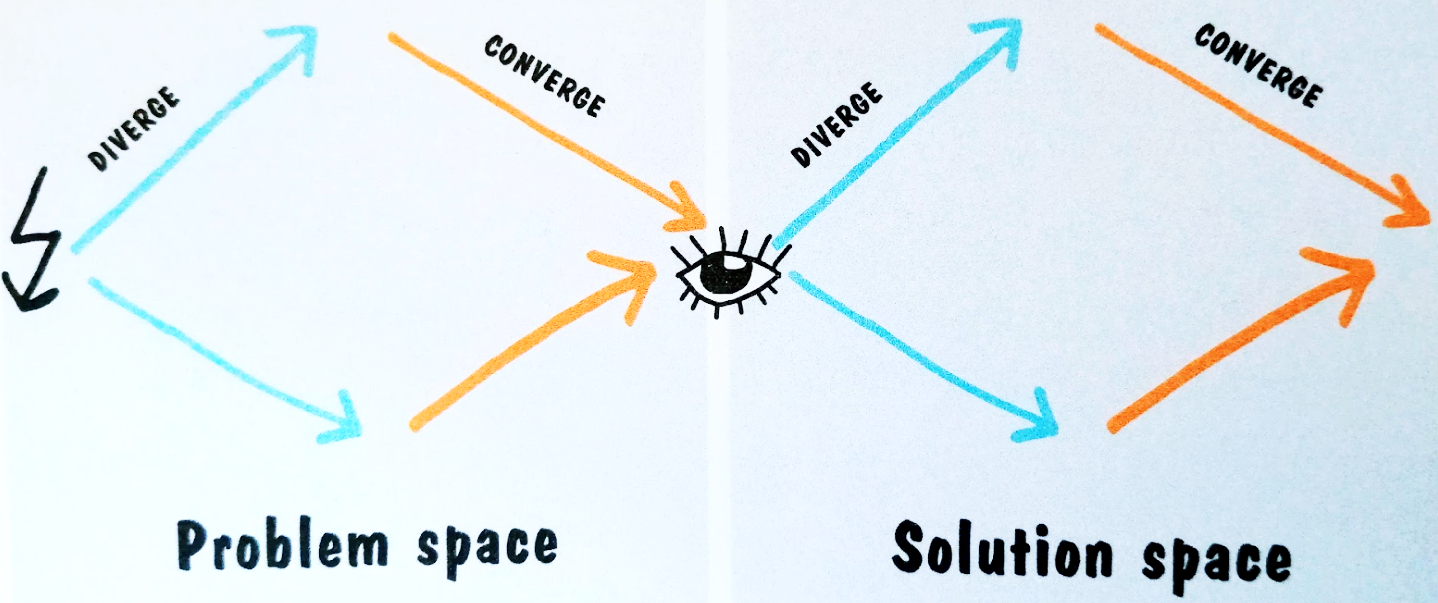
\includegraphics[width=\textwidth]{immagini/double-diamond.png}
\end{figure}

\section{Design Thinking}
Il Design Thinking è un approccio all’innovazione che poggia le sue fondamenta sulla capacità di risolvere problemi complessi utilizzando una visione e
una gestione del progetto basata sulla creatività. 

Tale approccio è stato codificato attorno agli anni 2000 in California dall’Università di Stanford. È centrato sulle persone (antropocentrico) e si
basa sull’abilità di integrare capacità analitiche con attitudini creative. In genere viene applicato da un team multidisciplinare che ha come
obiettivo quello di trovare una soluzione innovativa ad un problema (disruptive) tenendo conto del gradimento (Human-centered) di essa, della
redditività indotta e della sostenibilità economica (business).

In origine, il Design Thinking nacque come approccio all’innovazione adottato da agenzie e studi di design. Oggi invece, la sua diffusione sta
permeando in settori molto diversi, anche in quelli ritenuti più distanti, fino a qualche anno fa. Il design thinking sta diventando infatti uno dei
metodi di riferimento utilizzati dalle startup e da aziende innovative per la realizzazione di prodotti tecnologici, per la trasformazione digitale e
la progettazione di software e interfacce.

Il DT ha 3 obiettivi fondamentali:

\begin{enumerate}
	\itemsep-0.3em
	\item avvicinarsi al cliente;
	\item favorire la creatività e generare idee;
	\item sperimentare rapidamente le idee attraverso la realizzazione di prototipi.
\end{enumerate}

Tuttavia ridurre il DT all’elenco degli obiettivi, dei settori di utilizzo o dei tool che lo caratterizzano è estremamente limitante.
\`E invece molto più efficace ed importante comprendere il mindset e la prospettiva che caratterizzano i processi di DT. Questo perché
quotidianamente vengono proposti nuovi metodi, strumenti e tecnologie a supporto di questa modalità di progettazione e pertanto andare a trattarla
sulla base degli strumenti più utilizzati è scorretto e limitante.

\begin{figure}[!h]
	\centering
	\includegraphics[scale=0.35]{immagini/des_think.png}
\end{figure}

% Relativamente all'approccio DT, Roberto Verganti Professore di Leadership and Innovation alla Stockholm School of Economics afferma:
% \textit{Si tratta di ribaltare il classico triangolo, tipico delle business school, che pone nel vertice in alto il business e alla base people e
% technology, a indicare come l’obiettivo dell’impresa sia l’uso dell’innovazione per creare business value a favore degli stakeholder, grazie a
% prodotti che soddisfino i bisogni delle persone attraverso l’uso delle tecnologie.}

\textbf{L’approccio Design Thinking pone nel vertice in alto le persone.}
\textit{Partiamo dai sogni e dai problemi delle persone e creiamo prodotti che li soddisfino. Se ci riusciremo lo sviluppo del business ne sarà la
naturale conseguenza.}

\begin{figure}[!h]
	\centering
	\includegraphics[scale=0.25]{immagini/designthinking}
	\caption{Le 5 fasi del Design Thinking
	(\href{https://www.zerounoweb.it/cio-innovation/metodologie/design-thinking-definizione-esempi/}{\underline{Fonte}}).}
\end{figure}

In un processo di sviluppo basato su design thinking il business e la tecnologia sono solo degli strumenti per raggiungere l'obiettivo primo, la
soddisfazione dell'utente; si individuano le seguenti 5 fasi principali:

\begin{itemize}
	\itemsep-0.3em
	\item \textbf{Empathize}: La prima fase consiste nell’identificazione del problema e quindi dell’obiettivo; in questa fase si scrivono le personas.
	\item \textbf{Define}: La seconda fase è orientata a delineare meglio le domande chiave, cioè quali sono i bisogni degli utenti e quindi quali
	sono le varie categorie di utenti; in questa fase si lavora alle user stories e ai needs.
	\item \textbf{Ideate}: La terza fase è quella orientata alla ricerca della soluzione, dell'opportunità tecnologica. In questa fase si fa uso di
	tecniche di stimolazione della creatività come brainstorming etc. (per pensare alla soluzione).
	\item \textbf{Prototype}: La quarta fase è orientata alla realizzazione dei primi prototipi. Questa fase è molto importante per garantire un
	processo antropocentrico consentendo di andare il più velocemente possibile a testare il prodotto sul campo con gli utenti reali.
	L'implementation è intrinseca a questa fase.
	\item \textbf{Test}: In fine la quinta fase è quella dedicata al test sul campo dei prototipi e alla raccolta dei feedback dagli utenti.
	Questa fase apparentemente conclusiva in realtà produce come output una serie di input per i futuri cicli di iterazione che si vanno ad applicare
	a tutte le fasi precedenti.
\end{itemize}

Lo Human Centered Design è quindi un \textbf{mindset}, un modo di pensare e di approcciarsi allo sviluppo di prodotti. Come nel caso dello HCD
Process, il Design Thinking, è invece un vero e proprio metodo di lavoro organizzato per fasi che consente di sviluppare prodotti centrati sull'utente
grazie a tecniche orientate alla stimolazione della creatività e alla produzione di idee. Pensare di avviare un processo di disruptive innovation
senza curarsi di progettare in maniera antropocentrica e senza un metodo di progettazione strutturato è al giorno d'oggi impossibile.

\begin{figure}[!h]
	\centering
	\includegraphics[width=0.6\textwidth]{immagini/dtvshcdp}
\end{figure}

Human-Centered Design e Design Thinking sono compatibili e combinabili in un metodo detto \textbf{Social Enterprise Thinking}.

\begin{figure}[!h]
	\centering
	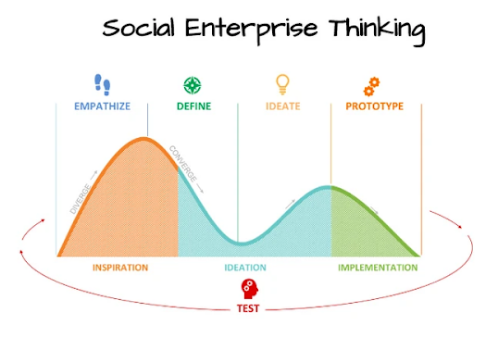
\includegraphics[scale=0.5]{immagini/social-enterprise-thinking.png}
\end{figure}

\section{Agile, Scrum e DevOps}
Nel mondo dello sviluppo software e dell'informatica in generale, negli utili anni si sono sviluppati molti metodi di organizzazione del lavoro
orientati allo sviluppo veloce di sistemi innovativi. Tanti di questi metodi si basano su un mix di teorie e approcci di design applicati in altri
settori e in generale puntano a dare al team di sviluppo un metodo di lavoro più snello, veloce e soprattutto orientato al prodotto e all'utente
(antropocentrico).

Il metodo di sviluppo software classico, presentato come fondamento dell'ingegneria del software è sicuramente il modello \textbf{Waterfall}.
In ingegneria del software, il modello a cascata (waterfall model in inglese) o ciclo di vita a cascata (waterfall lifecycle) è il più tradizionale
modello di ciclo di vita del software. Secondo questo modello, il processo di realizzazione del software è strutturato in una sequenza lineare di
fasi o passi, che comprende:

\begin{itemize}
	\itemsep-0.3em
	\item analisi dei requisiti;
	\item progettazione;
	\item sviluppo;
	\item collaudo;
	\item manutenzione.
\end{itemize}

Questo modello riprende la sequenza di passi tipica della produzione manifatturiera, e fu il primo a essere applicato all'informatica quando lo
sviluppo del software cominciò a essere concepito come attività industriale. Questo modello è stato progressivamente abbandonato dall'industria
del software, ma rimane un importante riferimento storico.

Uno dei nuovi modelli di organizzazione dello sviluppo software che negli ultimi anni sta riscuotendo maggior successo è sicuramente l’\textbf{Agile}.
Il metodo Agile nasce nel 2001 da un gruppo di 17 sviluppatori, che sentirono il bisogno di ripensare il loro modo di lavorare perchè stufi del
classico metodo di sviluppo Waterfall.
L'obiettivo di questi sviluppatori era quello di progettare un nuovo metodo di lavoro orientato allo sviluppo di applicazioni software in maniera più
leggera, economica e rapida (adattando il modello della Lean Manufacturing di Toyota).

\begin{figure}[h!]
	\centering
	\includegraphics{"immagini/agile_manifesto"}
\end{figure}

Produssero quindi un manifesto a partire dal quale sono stati sviluppati i 12 principi fondamentali dell'Agile:

\begin{enumerate}
	\itemsep-0.3em
	\item Our highest priority is to satisfy the customer through early and continuous delivery of valuable software.
	\item Welcome changing requirements, even late in development. Agile processes harness change for the customer's competitive advantage.
	\item Deliver working software frequently, from a couple of weeks to a couple of months, with a preference to the shorter timescale.
	\item Business people and developers must work together daily throughout the project.
	\item Build projects around motivated individuals. Give them the environment and support they need, and trust them to get the job done.
	\item The most efficient and effective method of conveying information to and within a development team is face-to-face conversation.
	\item Working software is the primary measure of progress.
	\item Agile processes promote sustainable development. The sponsors, developers, and users should be able to maintain a constant pace indefinitely.
	\item Continuous attention to technical excellence and good design enhances agility.
	\item Simplicity--the art of maximizing the amount of work not done--is essential.
	\item The best architectures, requirements, and designs emerge from self-organizing teams.
	\item At regular intervals, the team reflects on how to become more effective, then tunes and adjusts its behavior accordingly.
\end{enumerate}


I principi riportati nel manifesto focalizzano lo sviluppo del software sugli individui e le interazioni, sul prodotto realizzato piuttosto che
sulla documentazione, sull’interazione stretta con il cliente (utente) e soprattutto sui cambiamenti che possono avvenire anche durante lo sviluppo
stesso del prodotto o servizio.

In sostanza, nello sviluppo Agile, si procede con un team molto coeso, composto da product manager e sviluppatori, a definire i requirement per uno
sviluppo di una prima parte dell’applicazione, fermandosi poi a provare quanto realizzato, a ragionarci su e definire nuovi requirement per la
realizzazione di nuove funzioni o di una revisione di quanto realizzato.

Questa metodologia di sviluppo veloce e libero ha avuto una spinta notevole dall’avvento della tecnologia Cloud, che ha favorito il deploy continuo
del software consentendo quindi di velocizzare i cicli di sviluppo e test delle applicazioni.
Dalla Agile sono nate poi varie sotto-tecniche e metodi di organizzazione dello sviluppo software di cui lo \textbf{Scrum} è sicuramente una delle
più diffuse. 

Scrum si basa sulla teoria dei controlli empirici di analisi strumentale e funzionale di processo o empirismo. L'empirismo afferma che la conoscenza
deriva dall'esperienza e che le decisioni si basano su ciò che si conosce. Scrum utilizza un metodo interattivo ed un approccio incrementale per
ottimizzare la prevedibilità ed il controllo del rischio.
In maniera molto sintetica, Scrum è un framework di processo adatto a gruppi medio-piccoli (non più di 10 persone; se il team è particolarmente grosso,
allora si divide in più scrum team con focus diversi che avranno sessioni diverse ma si incontreranno periodicamente) che prevede di dividere il
progetto in blocchi rapidi di lavoro (i cosiddetti \textbf{Sprint}) alla fine di ciascuno dei quali creare un incremento del software. Esso indica
come definire i dettagli del lavoro da fare nell'immediato futuro e prevede vari meeting con caratteristiche precise per creare occasioni di
ispezione e controllo del lavoro svolto.

Il framework Scrum è profondamente antropocentrico. Ogni parte del framework serve a uno specifico scopo ed è essenziale per il successo e l'utilizzo
di Scrum. Le regole di Scrum legano insieme gli eventi, i ruoli e gli artefatti governando le relazioni e le interazioni tra essi anche se le
strategie specifiche per l'utilizzo del framework Scrum variano e vengono descritte in molti testi specifici.

Le persone che ricoprono i ruoli principali nel processo Scrum costituiscono il Team Scrum e sono quelle impegnate nel progetto e che realizzano il
prodotto (obiettivo del progetto). Il Team Scrum tiene traccia degli sviluppi con dei meeting giornalieri dalla durata di 15 minuti (detti
\textbf{daily scrum}); anche al termine degli Sprint vengono fatti dei meeting: \textbf{Sprint review} per mostrare i risultati ottenuti e
\textbf{Sprint retrospective} per fare il bilancio dello Sprint e migliorare in modo continuo.

\begin{figure}[h!]
	\centering
	\includegraphics[scale=0.5]{"immagini/Scrum-Agile-Marketing"}
	%\includegraphics[width=\textwidth]{"immagini/agile"}
\end{figure}

Il Team Scrum è formato dal Product Owner, Il Team di sviluppo (Development Team) e da uno Scrum Master.
\textbf{Il Product Owner rappresenta gli stakeholders ed è la voce del cliente.} È responsabile per assicurare che il team fornisca valore al business.
Il Product Owner definisce gli item (requisiti di prodotto) centrati sui bisogni dei clienti (HCD), assegna loro la priorità, e li
aggiunge al product backlog. I team Scrum debbono avere un Product Owner e si raccomanda che questo ruolo non sia combinato con quello dello
Scrum Master.
Lo \textbf{Scrum Master} non è il classico project manager, ma \textbf{organizza gli sprint e si assicura che il framework scrum venga seguito, ha
la responsabilità di guidare il team nel votare e valutare la complessità di ogni task}.

Il principio chiave è il riconoscimento che \textbf{i clienti cambieranno idea su cosa vogliano o di quali siano i loro bisogni} (si parla di
\textbf{requirements volatility}) e ci saranno dunque problemi non prevedibili o per i quali un approccio che prevede una pianificazione iniziale
non risulta adatto. \textbf{Scrum adotta un approccio basato sull'evidenza empirica}: accettando che \textbf{il problema non può essere del tutto
compreso o definito} e concentrandosi sul come massimizzare le abilità del team per \textbf{consegnare velocemente e rispondere a cambiamenti nei
requisiti e adattarsi a cambiamenti sia sul piano tecnologico sia di mercato}.

\begin{figure}[h!]
	\centering
	\includegraphics[width=0.5\textwidth]{"immagini/devops-process"}
	\caption{Ciclo DevOps (\href{https://italiancoders.it/introduzione-al-devops/}{\underline{Fonte}}).}
\end{figure}

L'integrazione dei metodi Agile con il mondo del cloud, dei micro servizi e della programmazione server-less ha portato negli ultimi anni (2009)
alla nascita di un nuovo metodo di sviluppo DevOps.

Il DevOps prevede, attraverso la collaborazione e integrazione tra sviluppatori e addetti alle operation la gestione più flessibile, affidabile,
sicura e controllabile dei rilasci, tale da rendere più veloci i cicli di sviluppo e rilascio. Il DevOps si ispira alla metodologia Agile, alla
necessità di incrementare la frequenza dei rilasci in produzione e fa leva sulla disponibilità di infrastrutture virtualizzate e in cloud.

% \section{Analisi delle Cause Profonde}
% \begin{flushleft}
% 	\href{https://www.tableau.com/it-it/learn/articles/root-cause-analysis}{\underline{Fonte}}.
% \end{flushleft}
% 
% La Agile e la Scrum abbiamo detto essere delle tecniche basate su cicli di sviluppo e verifica basati su un forte impianto empiristico. queste tecniche prevedono quindi che una volta sviluppato del software si eseguano dei test, si analizzino i problemi e si lavori per risolvere le cause che hanno generato i malfunzionamenti identificati o hanno comportato frustrazione nel cliente/utente.
% 
% L'identificazione delle cause di un problema sembra un processo banale ma in realtà è un'attività estremamente complessa. Spesso infatti, si tende a confondere il problema con il sintomo che questo comporta. e' tipicamente semplice eliminare il sintomo ma è spesso molto complesso eliminare la causa.
% 
% \textit{Se avete la tosse, prenderete una caramella al miele vi passerà la tosse (il sintomo) per qualche minuto ma poi la tosse tornerà perchè la causa scatenante non è stata rimossa e quindi il problema è ancora presente e il sintomo si ripresenterà.}
% 
% L'analisi delle cause profonde (RCA, Root cause analysis) è un procedimento finalizzato all'identificazione delle cause poste alla radice di un problema. L'obbiettivo della RCA è quindi quello di risolvere i problemi all'origine andando oltre la semplice tacitazione dei sintomi. L'RCA parte dal presupposto che sia molto più utile prevenire e risolvere le problematiche sottostanti in modo sistematico invece di trattare semplicemente i sintomi e arginare il problema caso per caso.
% 
% La RCA è quindi uno strumento fondamentale per la gestione dei processi di sviluppo di tipo Agile.
% 
% L'analisi delle cause profonde può essere eseguita con l'aiuto di vari principi, tecniche e metodologie da mettere in pratica per identificare le cause alla radice di un evento o di un trend. L'RCA scava più a fondo della causa e dell'effetto in superficie ed è in grado di evidenziare le lacune dei processi e dei sistemi o il motivo alla base dell'insorgenza di un problema.
% 
% Obiettivi e vantaggi della RCA:
% \begin{enumerate}
%     \item Il primo obiettivo dell'analisi delle cause profonde è scoprire la causa all'origine di un problema o di un evento.
%     \item Il secondo obiettivo è comprendere appieno come correggere e trovare un rimedio alle problematiche sottostanti all'interno della causa principale, oltre a imparare da queste.
%     \item Il terzo obiettivo è applicare quanto imparato da questa analisi per impedire in modo sistematico problematiche future o per ottenere di nuovo risultati positivi.
% 
% \end{enumerate}
% 
% Ciò che facciamo con i risultati di questa analisi è importante quanto l'analisi stessa e quindi il terzo obiettivo ha una rilevanza da non sottovalutare. Possiamo utilizzare l'RCA anche per modificare le problematiche principali dei processi e dei sistemi in modo da evitare che si verifichino problemi in futuro. Invece di trattare semplicemente i sintomi di una commozione cerebrale di un rugbista, ad esempio, l'analisi delle cause profonde può suggerire di fargli indossare un caschetto per ridurre il rischio di traumi futuri.
% 
% Trattare i sintomi uno per uno può sembrare produttivo e risolvere un ampio numero di problemi dà l'impressione di aver trovato una soluzione efficace (tipico dei processi di debug del software). Tuttavia, se ignoriamo la diagnosi effettiva della vera causa scatenante, lo stesso identico problema potrebbe ripresentarsi ancora e ancora. 
% 
% Invece di incaricare un redattore di correggere ogni singola virgola omessa, insegnare agli scrittori a usare correttamente la punteggiatura permetterebbe di non affrontare più queste problematiche in testi futuri.
% 
% Alla base di un'efficace analisi delle cause profonde vi sono alcuni principi chiave, che in parte dovrebbero già essere evidenti. Questi non solo contribuiscono alla qualità dell'analisi, ma aiutano anche gli analisti a creare fiducia e ottenere l'approvazione di parti interessate, clienti o pazienti.
% 
% \begin{itemize}
%     \item Punta a risolvere e trovare una soluzione per le cause profonde, non per i soli sintomi.
%     \item Non ignorare l'importanza di trattare i sintomi per una soluzione a breve termine.
%     \item Considera il fatto che possono esserci, e spesso ci sono, più cause profonde.
%     \item Concentrati sul COME e sul PERCHÉ si è verificato un evento, non sul CHI ne è responsabile.
%     \item Adotta un approccio metodico e trova le prove concrete della relazione di causa-effetto per avere una conferma delle cause profonde rilevate.
%     \item Fornisci informazioni sufficienti per dare forma a un percorso di azioni correttivo.
%     \item Valuta come evitare l'insorgenza (o il ripetersi) di una causa profonda in futuro.
% 
% \end{itemize}
% 
% Come risulta chiaro da questi principi, quando analizziamo le problematiche e le cause profonde, è importante adottare un approccio onnicomprensivo e olistico. Oltre a scoprire la causa profonda, dobbiamo fare in modo di raccogliere dati contestuali e informazioni sufficienti per intraprendere un'azione correttiva o prendere una decisione; \textbf{una buona analisi è un'analisi attuabile.}
% 
% Le tecniche e le strategie per l'analisi delle cause profonde sono numerosissime, il metodo dei 5 perchè è uno dei più utilizzati e semplici da capire.
% 
% \subsection{Metodo dei 5 Perché}
% Una delle tecniche più seguite per effettuare un'analisi delle cause profonde è il metodo dei 5 Perché. È più o meno quello che succede quando i bambini chiedono tutti quei fastidiosi perché uno dietro all'altro, dove a ogni domanda ne segue un'altra concatenata e che scava sempre più a fondo. I bambini sono sorprendentemente bravi con l'analisi delle cause profonde. L'opinione diffusa è che siano sufficienti circa cinque PERCHÉ per identificare le principali cause profonde, ma potrebbero volercene un po' di meno o molti di più.
% 
% \textbf{Esempio:} prendiamo di nuovo l'esempio della commozione cerebrale del rugbista. \\
% 
% Prima di tutto, il giocatore solleva un problema: perché ho questo terribile mal di testa? Questo è il nostro primo PERCHÉ.
% Prima risposta: perché ci vedo doppio.\\
% 
% Secondo perché: perché ci vedi doppio?
% Seconda risposta: perché ho sbattuto la testa a terra.\\
% 
% Terzo perché: perché hai sbattuto la testa a terra?
% Terza risposta: sono stato placcato e ho sbattuto la testa a terra.\\
% 
% Quarto perché: perché cadere a terra ti ha fatto così male?
% Quarta risposta: perché non indossavo il caschetto.\\
% 
% Quinto perché: perché non indossavi un caschetto?
% Quinta risposta: perché non c'erano abbastanza caschetti nello spogliatoio.
% 
% Ecco, dopo queste cinque domande abbiamo scoperto che la causa alla radice della commozione cerebrale è molto probabilmente una mancanza di caschetti disponibili. Per il futuro, possiamo ridurre il rischio di traumi di questo genere assicurandoci che ogni giocatore abbia un caschetto.
% 
% \textbf{Il metodo dei 5 Perché ci permette di non fare supposizioni}. Man mano che aumentano le domande, le risposte dettagliate diventano sempre più chiare e concise. In teoria, l'ultimo PERCHÉ porta a identificare una lacuna nel processo, che quindi può essere corretta.
 %Metodi e Strumenti per l'Innovazione

%\include{capitoli/capitolo_12}
%\include{capitoli/capitolo_13}
\chapter{Pretotipazione delle interfacce}
\begin{figure}[!h]
	\centering
	\includegraphics[scale=0.5]{immagini/Fall_mercato.png}
\end{figure}

Un prodotto \textbf{pretotipo} serve a lottare contro la legge di fallimento di mercato. Ogni anno vengono progettati e prodotti quasi 25000 nuovi prodotti
l'80\% dei quali non vedrà mai la luce o non arriverà mai nelle case delle persone. Circa il 27\% falliscono nel percorso di crescita dell'azienda, il
16\% non raggiunge le aspettative degli utenti, trattasi quindi di fallimento di mercato, e per ben il 37\% vengono cancellati durante la fase di lancio.
Del 20\% rimanente, il 14\% sono prodotti che raggiungo il mercato e ci rimangono ma non hanno successo. \textbf{Solo il 6\% ha veramente successo}.

\begin{figure}[!h]
	\centering
	\includegraphics[scale=0.15]{immagini/legge-fallimento-di-mercato.png}
\end{figure}

La \textbf{legge del fallimento di mercato sostiene che la maggior parte dei nuovi prodotti fallirà nel mercato anche se la progettazione e lo sviluppo
vengono eseguite in maniera corretta e competente}. In legge, una persona è considerata innocente fino a prova contraria, mentre nella legge di mercato,
\textbf{bisogna considerare ogni prodotto come fallito fino a prova contraria}.

Esiste una e una sola tecnica per sconfiggere la legge di fallimento di mercato: testare in modo oggettivo, rigoroso e rapido le proprie idee sul mercato
prima di investire per svilupparle; la \textbf{pretotipazione} fornisce strumenti e tecniche per validare le proprie idee con risorse minime e nel minor
tempo possibile.

\pagebreak

\begin{figure}[!h]
	\centering
	\includegraphics[scale=0.25]{immagini/innovation-fast-testing.png}
\end{figure}

\section{Thoughtland, il mondo dei pensieri}
Quando si progetta un nuovo prodotto, o si ha semplicemente un'idea, ci si trova di fronte a \textbf{due grandi problemi}: il \textbf{lost in translation}
e \textbf{il problema della predizione}. Il primo si ha quando l'idea è un'astrazione soggettiva, qualcosa che si può immaginare o visualizzare in testa.
Nel momento in cui si prova a comunicarla a qualcun altro però, si incontra un problema di traduzione, specialmente quando l'idea è nuova ed è diversa da
qualsiasi altra cosa abbia visto l'interlocutore.

Il modo in cui si immagina un nuovo prodotto e i suoi usi può essere completamente diverso da come gli altri lo immaginano a loro volta. Si può ovviare
utilizzando \textbf{termini noti}, infatti è molto difficile veicolare il modello concettuale all'utente. L'altro problema è conosciuto come il
\textbf{problema della predizione}: anche se la comprensione astratta dell'idea che l'interlocutore ha è molto vicina alla propria, egli in quanto essere
umano è molto \textbf{scarso per sua natura} nel prevedere se essa potrebbe essere di suo gradimento o meno.

\section{Thoughts without data are just opinions}
\begin{flushleft}
	\textit{I pensieri senza dati sono solo opinioni.}
\end{flushleft}

Questa è una delle più importanti frasi da tenere presente quando si pensa di lanciare nuovi oggetti o idee nel mercato, anche se è spesso sottovalutata.

I falsi positivi possono portare a credere che l'idea sia immune alla legge del fallimento di mercato, e quindi a investire troppo e presto in un prodotto
che probabilmente fallirà.

I falsi negativi possono invece spaventare e portare a non concedere una chance all'idea, finendo per scartare prematuramente il prossimo Twitter, Google o
Tesla.

Per poter minimizzare la possibilità di ottenere falsi positivi o negativi è necessario \textbf{uscire dal Thoughtland}, quindi dal mondo delle idee
astratte e delle opinioni, e \textbf{muoversi verso l'Actionland}, dove si usano \textbf{artefatti} per collezionare dati e osservare le azioni degli
utenti. Nel primo caso si usano le domande o questionari per poter ottenere informazioni sul prodotto che si andrà a sviluppare, col rischio di collezionare
opinioni poco utili e magari fuorvianti, nel secondo caso, mediante artefatti, si fanno svolgere azioni agli utenti al fine di raccogliere dati.

I prodotti del Thoughtland sono: \textbf{idee}, \textbf{domande} e \textbf{opinioni}. Quelli dell'Actionland sono \textbf{artefatti}, \textbf{azioni} e
\textbf{dati}.

\pagebreak

\begin{figure}[!h]
	\centering
	\includegraphics[scale=0.6]{immagini/Manifesto.png}
\end{figure}

\begin{figure}[!h]
	\centering
	\includegraphics[scale=0.25]{immagini/pretotyping-manifesto-corollario.png}
	\caption{Corollario del manifesto.}
\end{figure}

\section{Pretotype vs Prototype}
I prototipi aiutano a fallire in fretta, ma spesso non abbastanza in fretta o non abbastanza economicamente.
Più si investe in un'idea e \textbf{più diventa difficile lasciarla morire} e ammettere che era sbagliata, anzi tendenzialmente, una volta ottenuto un buon
prototipo che funziona, è facile portarlo avanti investendovi ancora denaro e tempo, pensando che l'aggiunta di funzionalità e features sia la risposta per
renderlo vincente. Molto spesso i prodotti lanciati sul mercato non sono altro che prototipi andati troppo oltre. \textbf{Tra il mondo delle idee astratt
 e i prototipi funzionanti}, si collocano i \textbf{pretotypes}.

\textbf{Un pretotipo è un semplice mockup del prodotto che si vorrebbe sviluppare} ed è utile per ottenere sia informazioni d'uso che di mercato e,
specialmente, per poter prendere decisioni su cosa fare e su cosa non fare.

La \textbf{principale differenza} tra un pretotipo e un prototipo è l'\textbf{investimento}: un \textbf{pretotipo costa molto meno} sia in termini di tempo 
che in termini di denaro, e consente di fallire in fretta o nel caso, poiché lascia un ampio spazio di manovra, di apportare modifiche.

\begin{figure}[!h]
	\centering
	\includegraphics[scale=0.45]{immagini/Pre_prot.png}
\end{figure}

Lo scopo è quello di investire minuti, ore o giorni anziché settimane, mesi o anni.

Il \textbf{pretotyping} ha l'obiettivo di aiutare a:

\begin{itemize}
	\itemsep-0.3em
	\item \textbf{Identificare le funzionalità chiave} del nuovo prodotto.
	\item Decidere \textbf{quali} di queste possono o dovrebbero essere \textbf{inserite nel mockup}.
	\item Usare i mockups per il \textbf{test sistematico} e contemporaneamente \textbf{collezionare feedback e dati d'uso}.
	\item Analizzare i dati raccolti per \textbf{determinare il prossimo passo da compiere}.
\end{itemize}

I \textbf{sette pilastri del Pretotyping} sono:

\begin{enumerate}
	\itemsep-0.3em
	\item \textbf{Obbedire alla Legge del Fallimento di Mercato}.
	\item \textbf{Assicurarsi di star costruendo il prodotto giusto}.
	\item \textbf{Non perdersi in chiacchiere, idee o opinioni}.
	\item \textbf{Fidarsi solo dei propri dati, \textbf{TRUST YODA: Your Own DAta}}.
	\item \textbf{Fare pretotyping}.
	\item \textbf{Parlare con i numeri e con i fatti}.
	\item \textbf{Pensare globalmente, testa localmente}.
\end{enumerate}

\section{Flusso del Pretotyping}

I \textbf{cinque step} per produrre un buon pretotipo sono i seguenti:

\begin{enumerate}
	\itemsep-0.3em
	\item \textbf{Isolare l'assuzione chiave}: qual è la assunzione o funzionalità chiave dell'idea che, se falsa, ne minerebbe la validità?
	\item \textbf{Scegliere un tipo di pretotype}: quale tipo di pretotyping permette di isolare e testare al meglio le funzionalità chiave?
	\item \textbf{Fare ipotesi di mercato}: quante e quali tipi di persone utilizzeranno il pretotipo (si parla di \textbf{ipotesi XYZ}: almeno X\% di Y
	farà Z)? Come lo utilizzeranno? Sarebbe possibile ipotizzare le percentuali di un determinato utilizzo?
	\item \textbf{Testare il pretotype}: mettere il pretotipo nel mondo reale e vedere quante persone sono interessate e quante ci interagiscono. Bisogna
	partire dal basso, un passo alla volta.
	\item \textbf{Imparare, rifinire, hypozoom}: valutare i risultati, rifinire il pretotipo con i nuovi dati, e se l'ipotesi ha retto, decidere quali altre
	situazioni testare per ottenere man mano una \textbf{visione completa}: \textbf{hypozooming}, \textbf{think global}, \textbf{test local}.
\end{enumerate}

\section{Tipi di Pretotyping}
Andiamo ad analizzare alcuni tipi di pretotyping.
\begin{itemize}
	\item Una \textbf{Fake Door} è un marketing entry point per un prodotto che ancora \textbf{non esiste} e può essere utilizzata per \textbf{pubblicizzare}
	un servizio non ancora pronto e misurare l'interesse degli utenti.

	È un buon modo per capire se l'oggetto che si vuole sviluppare può avere successo o meno, spendendo pochissimo e quindi, in caso di fallimento, avere
	un basso impatto economico, inteso sempre sia in termini di denaro che di tempo. Si può usare questo tipo di pretotyping \textbf{quando l'idea può
	essere descritta in poche e semplici parole}, senza possedere nulla di fisico o materiale.
	\pagebreak
	\begin{figure}[!h]
		\centering
		\includegraphics[scale=0.42]{immagini/Fake_door.png}
	\end{figure}

	\item Si parla di \textbf{Mechanical Turk} quando ci si riferisce ad un oggetto che riesce, nel suo utilizzo, a trasmettere l'esperienza del prodotto
	finale ad un utente, senza che sia stato sviluppato. Un mechanical turk usa solo man power. È molto utilizzato per sperimentare l'uso e la reale
	applicabilità di software e algoritmi molto costosi per essere implementati.
	\begin{figure}[!h]
		\centering
		\includegraphics[scale=0.42]{immagini/Mechanical_turk.png}
	\end{figure}

	\item Un \textbf{Impersonator} è un pretotipo che riesce a far sperimentare un'esperienza realistica all'utente in modo estremamente economico e con
	un lavoro minimo dietro. Consente cioè di far vivere l'esperienza esattamente come se il prodotto fosse finito e pronto per essere lanciato.
	\begin{figure}[!h]
		\centering
		\includegraphics[scale=0.42]{immagini/Impersonator.png}
	\end{figure}

	\item Un \textbf{Pinocchio} è un pretotipo \textbf{chiaramente falso}, serve per veicolare un messaggio così distante dalla realtà attuale che è
	faticoso e difficile da spiegare in altri linguaggi naturali. È usato molto spesso per testare l'interesse e il possibile uso di prodotti innovativi
	e non ancora lanciati da nessuno, nemmeno in maniera simile, sul mercato.
	\pagebreak
	\begin{figure}[!h]
		\centering
		\includegraphics[scale=0.5]{immagini/Pinocchio.png}
	\end{figure}

	\item Con \textbf{One Night Stand} si indica una \textbf{tecnica di veicolazione} di un pretotipo. Consiste di un \textbf{market test}.
	Viene usato insieme ad un'altra tecnicha di pretotyping per veicolare meglio il messaggio a una certa cerchia di persone.
	\begin{figure}[!h]
		\centering
		\includegraphics[scale=0.5]{immagini/One_night_stand.png}
	\end{figure}

	\item Un \textbf{Facade} è una sorta di Impersonator ma è usato per dare un'immagine dell'azienda e non del prodotto stesso. Viene sfruttato spesso
	per promuovere servizi.
	\begin{figure}[!h]
		\centering
		\includegraphics[scale=0.5]{immagini/Facade.png}
	\end{figure}

\end{itemize}

\pagebreak

\section{Minimum Viable Product}

Dopo varie fasi di pretotyping e aver accumulato sicurezze sufficienti circa il successo del prodotto, lo step successivo è produrre il
\textbf{Minimum Viable Product}, cioè la \textbf{versione minimale del prodotto contenente solo ed esclusivamente le features che si sono pretotipate
attraverso la fase precedente}. Non si ha ancora per le mani un prodotto definitivo besì un qualcosa di \textbf{vendibile}, in modo da ottenere del ricavo
e dell'utile, che se sufficiente, permetterebbe la produzione definitiva del prodotto.

\begin{figure}[!h]
	\centering
	\includegraphics[scale=0.4]{immagini/MVP.png}
	\caption{Minimum Viable Product.}
	\includegraphics[scale=0.4]{immagini/ONS.png}
	\includegraphics[scale=0.4]{immagini/Pnocc.png}
	\caption{A sinistra esempi di one night stands e a destra esempi di pinocchio.}
	\includegraphics[scale=0.6]{immagini/Imp.png}
	\caption{Esempi di Impersonator.}
\end{figure}

\pagebreak

 %pretotyping

\end{document}